%\documentclass[aps,prl,preprint,superscriptaddress,showpacs]{revtex4}
\documentclass[aps,prl,reprint,longbibliography,superscriptaddress, english]{revtex4-1}
%\documentclass[aps,prl,reprint,longbibliography]{revtex4-1}
%\usepackage{graphicx}
 \usepackage[utf8]{inputenc}
 \usepackage{amsmath,bm}
 \usepackage{mathrsfs}
 \usepackage{amsfonts}
 %\usepackage[font=it]{caption}
 \usepackage{graphicx}
 %\usepackage{xcolor}
 \usepackage{setspace} %leaves captions single space in draft mode
 \usepackage{graphicx}
 \usepackage{epstopdf}
 \usepackage{dcolumn}
 \usepackage{amsmath}
 \usepackage{epsfig}
 \usepackage{indentfirst}
 \usepackage{psfrag}
 \usepackage[normalem]{ulem}
 \usepackage{subfigure}
 %\usepackage{subcaption}
 \usepackage{amssymb}
 %\bibliographystyle{apsrev}
 \usepackage{color}
 \usepackage{units} % rz
\usepackage{soul} % strikethrough text
\usepackage{siunitx}
 \usepackage{graphicx}% Include figure files
 \usepackage{float}
 \graphicspath{{Figures/}} %Setting the graphicspath
 \usepackage{dcolumn}% Align table columns on decimal point
 \usepackage{bm}% bold math
 \usepackage{multirow}

\usepackage{physics}
\usepackage{dcolumn}% Align table columns on decimal point
\usepackage{bm}% bold mathhttps://www.overleaf.com/project/5af95d0f3775594d14d4a052
%\usepackage{hyperref}% add hypertext capabilities
\usepackage{natbib}
\usepackage[backref=none,bookmarksnumbered=true,bookmarks=true,bookmarksopen=true,colorlinks=true,
citecolor=blue,linkcolor=blue,anchorcolor=green,urlcolor=blue,unicode=false]{hyperref}

%******************************* For corrections ===================
\usepackage{ulem}[normalem] %Whatch out, places underlining in Journal references. Use \normalem before references to deactivate this 
\def\red{\color{red}}
\def\black{\color{black}}
\def\blue{\color{blue}}
\def\BappCl{BaCl$_2$}
%\def\Bapp{Ba$^{+2}$ }
%\def\Nap{Na$^{+}$ }


\normalem
\newcommand{\np}[1]{\textcolor{blue}{ #1}}
\newcommand{\npc}[1]{\textcolor{cyan}{(NP: #1)}}
\newcommand{\rw}[1]{\textcolor{cyan}{RW: #1}}
\newcommand{\str}[1]{\textcolor{cyan}{\st{#1}}}

\newcommand{\completar}[1]{{\color{red} #1}}
\newcommand{\rev}[1]{{\color{blue} #1}}

\makeatletter
\newcommand\colorsout[1]{\bgroup \markoverwith{\textcolor{#1}{\rule[0.5ex]{2pt}{0.4pt}}}\ULon}
\newcommand{\effacer}[1]{{\colorsout{red}{{\color{red}#1}}}}
\makeatother
%******************************* For corrections ===================

%******************************* Supporting Info ===================
\newcommand{\beginsupplement}{%
        \setcounter{table}{0}
        \renewcommand{\thetable}{S\arabic{table}}%
        \setcounter{figure}{0}
        \renewcommand{\thefigure}{S\arabic{figure}}%
     }
%******************************* Supporting Info ===================


%\usepackage{siunitx}
%\sisetup{separate-uncertainty=true}
%\usepackage{xspace}

\newcommand{\BF}[1]{\textbf{#1}\xspace}
\newcommand{\ITA}[1]{\textit{#1}\xspace}

%REFS
\newcommand{\sDIPC}{COORD}
\newcommand{\sIFIC}{MEAN}
\newcommand{\sUSC}{CALMU}
\newcommand{\sUPV}{SENSE}
\newcommand{\NEW}{NEXT-White}
\newcommand{\NEXT}{NEXT-100}
\newcommand{\REFS}{\textbf{REFS}}
\newcommand{\fig}{figure}
\newcommand{\eq}{equation}
\newcommand{\tab}{table}
\newcommand{\Fig}{Figure}
\newcommand{\Eq}{Equation}
\newcommand{\Tab}{Table}
\newcommand{\eg}{{\it e.g.}}
\newcommand{\ie}{{\it i.e.}}

\newcommand{\XenonLamp}{\SI{365}{nm}}
\newcommand{\FBIE}{\SI{250}{nm}}
\newcommand{\SFC}{\SI{2.3E-5}{\milli\mol}}
\newcommand{\SFD}{\SI{7.4E-8}{\milli\mol}}
\newcommand{\NFD}{\num{1.3E+15}}
\newcommand{\NSUB}{\num{7.6E+14}}
\newcommand{\BandFilter}{\ensuremath{\rm (400-425)~ nm}}
\newcommand{\GibbsP}{\SI{-80.0}{ kcal/mol}}
\newcommand{\GibbsPN}{-80.0}
\newcommand{\GibbsSB}{\SI{-195.9}{ kcal/mol}}
\newcommand{\GibbsBa}{\SI{-197.5}{ kcal/mol}}
\newcommand{\BaPer}{\ensuremath{\rm Ba(ClO_4)_2}}
\newcommand{\CHCN}{\ensuremath{\rm CH_3CN}}
\newcommand{\blt}{\ensuremath{\bullet}}
\newcommand{\xmus}{\ensuremath{x^{\mu}}}
\newcommand{\xmul}{\ensuremath{x_{\mu}}}
\newcommand{\xnus}{\ensuremath{x^{\nu}}}
\newcommand{\xnul}{\ensuremath{x_{\nu}}}
% stats
\newcommand{\micro}{\ensuremath{\mu}}
\newcommand{\chitwo}{\ensuremath{\chi^2}}
\newcommand{\NGA}{\ensuremath{n_\gamma}}
\newcommand{\stat}{\textrm{(stat.)}}
\newcommand{\sys}{\textrm{(sys.)}}
% BB\becquerel
\newcommand{\bb}{\ensuremath{\beta\beta}}
\newcommand{\nph}{\ensuremath{n_\gamma}}
% BB0NU
\newcommand{\bbonu}{\ensuremath{\beta\beta0\nu}}
% BB2NU
\newcommand{\bbtnu}{\ensuremath{\beta\beta2\nu}}
% NME
\newcommand{\Mnuc}{\ensuremath{M_{nuc}}}
\newcommand{\Monu}{\ensuremath{\Big|M_{0\nu}\Big|}}
\newcommand{\Mtnu}{\ensuremath{\Big|M_{2\nu}\Big|}}
% PHASE-SPACE FACTOR
\newcommand{\Gonu}{\ensuremath{G_{0\nu}(\Qbb, Z)}}
\newcommand{\Gtnu}{\ensuremath{G_{2\nu}(\Qbb, Z)}}
\newcommand{\tz}{\ensuremath{t_0}}
\newcommand{\stwo}{\ensuremath{S_2}}
\newcommand{\sone}{\ensuremath{S_1}}
\newcommand{\tyear}{\ensuremath{ton\cdot year}}

% mbb
\newcommand{\mbb}{\ensuremath{m_{\beta\beta}}}
\newcommand{\kgy}{\ensuremath{\rm kg \cdot y}}
\newcommand{\ckky}{\ensuremath{\rm counts/(keV \cdot kg \cdot y)}}
\newcommand{\mbba}{\ensuremath{m_{\beta\beta}^a}}
\newcommand{\mbbb}{\ensuremath{m_{\beta\beta}^b}}
\newcommand{\mbbt}{\ensuremath{m_{\beta\beta}^t}}
\newcommand{\nbb}{\ensuremath{N_{\beta\beta^{0\nu}}}}

%gases
\newcommand{\NIT}{\ensuremath{N_2}}
% Qbb
%\newcommand{\Qbb}{\ensuremath{Q_{\beta\beta}}}
\newcommand{\Qbb}{\ensuremath{Q}}

%%% U-238
\newcommand{\URANIUM}{\ensuremath{^{238}\mathrm{U}}}
%%%% Th-232
%\newcommand{\THORIUM}{\ensuremath{^{232}\mathrm{Th}}}
% Tonu
\newcommand{\Tonu}{\ensuremath{T_{1/2}^{0\nu}}}

% T2nu
\newcommand{\Ttnu}{\ensuremath{T_{1/2}^{2\nu}}}

% Cs-137
\newcommand{\CS}{\ensuremath{^{137}}Cs}

% Na-22
\newcommand{\NA}{\ensuremath{^{22}}Na}

% Ag-110
\newcommand{\AG}{\ensuremath{^{110m}}Ag}


% Bi-214
\newcommand{\RATT}{\ensuremath{^{226}}Ra}
%\newcommand{\Bi}{\ensuremath{^{214}}Bi}

% Tl-208
%\newcommand{\Tl}{\ensuremath{^{208}}Tl}


\newcommand{\KR}{\ensuremath{^{83m}\mathrm{Kr}}\xspace}


% Th-228
%\newcommand{\Th}{\ensuremath{^{228}}Th}
%\newcommand{\THO}{\ensuremath{^{228}}Th}
% Th-232
%\newcommand{\232Th}{\ensuremath{^{232}}Th}

% Pb-208
\newcommand{\PB}{\ensuremath{^{208}}Pb}
% Pb-208
\newcommand{\PBD}{\ensuremath{^{210}}Pb}

% Po-214
\newcommand{\PO}{\ensuremath{^{214}}Po}

% Rn-222
\newcommand{\RAD}{\ensuremath{^{222}}Rn}

% bru
\newcommand{\bru}{cts/(keV$\cdot$kg$\cdot$y)}

% Saltos de carro en tablas
\newcommand{\minitab}[2][l]{\begin{tabular}{#1}#2\end{tabular}}

\newcommand{\thedraft}{0.1.1}% version for referees

\newcommand{\SEVEN}{\ensuremath{\textbf{7}}}
\newcommand{\FPEAK}{\ensuremath{f_\lambda}}
\newcommand{\SEVENBA}{\textbf{7}$\cdot Ba^{2+}$}
\newcommand{\MO}{\ensuremath{{}^{100}{\rm Mo}}}
\newcommand{\SEL}{\ensuremath{{}^{82}{\rm Se}}}
\newcommand{\ZR}{\ensuremath{{}^{96}{\rm Zr}}}
%\newcommand{\KR}{\ensuremath{{}^{83m}{\rm Kr}}}
\newcommand{\ND}{\ensuremath{{}^{150}{\rm Nd}}}
\newcommand{\XE}{\ensuremath{{}^{136}\rm Xe}}
\newcommand{\GE}{\ensuremath{{}^{76}\rm Ge}}
\newcommand{\GES}{\ensuremath{{}^{68}\rm Ge}}
\newcommand{\TE}{\ensuremath{{}^{128}\rm Te}}
\newcommand{\TEX}{\ensuremath{{}^{130}\rm Te}}
\newcommand{\TL}{\ensuremath{{}^{208}\rm{Tl}}}
\newcommand{\CA}{\ensuremath{{}^{48}\rm Ca}}
\newcommand{\CO}{\ensuremath{{}^{60}\rm Co}}
\newcommand{\COFiftySix}{\ensuremath{{}^{56}\rm Co}}
\newcommand{\COFiftySeven}{\ensuremath{{}^{57}\rm Co}}
%\newcommand{\PO}{\ensuremath{{}^{214\rm Po}}}
%\newcommand{\U}{\ensuremath{{}^{235}\rm U}}
\newcommand{\CT}{\ensuremath{{}^{10}\rm C}}
\newcommand{\BE}{\ensuremath{{}^{11}\rm Be}}
\newcommand{\BO}{\ensuremath{{}^{8}\rm Be}}
\newcommand{\UDTO}{\ensuremath{\rm {}^{238}\rm U}}
\newcommand{\CD}{\ensuremath{^{116}{\rm Cd}}}
\newcommand{\THO}{\ensuremath{\rm {}^{232}{\rm Th}}}
\newcommand{\TO}{\ensuremath{\rm {}^{228}}Th}
\newcommand{\RADO}{\ensuremath{^{224}}Ra}
\newcommand{\BI}{\ensuremath{{}^{214}}Bi}
\newcommand{\Bapp}{\ensuremath{{\rm Ba^{2+}}}}
\newcommand{\Bap}{\ensuremath{\rm Ba^{+}}}
\newcommand{\Rapp}{\ensuremath{\rm Ra^{2+}}}
\newcommand{\Capp}{\ensuremath{Ca^{++}}}
\newcommand{\Srpp}{\ensuremath{\rm Sr^{2+}}}
\newcommand{\Mgpp}{\ensuremath{\rm Mg^{2+}}}
\newcommand{\Kp}{\ensuremath{\rm K^{+}}}
\newcommand{\Nap}{\ensuremath{\rm Na^{+}}}
\newcommand{\CHF}{\ensuremath{\rm CH_4}}
\newcommand{\RATX}{\ensuremath{\rm {}^{228}}Ra}

% alternative (clearer) definitions

\newcommand{\Ba}[1]{\ensuremath{^{#1}\mathrm{Ba}}\xspace}
\newcommand{\Bi}[1]{\ensuremath{^{#1}\mathrm{Bi}}\xspace}
\newcommand{\Co}[1]{\ensuremath{^{#1}\mathrm{Co}}\xspace}
\newcommand{\Cs}[1]{\ensuremath{^{#1}\mathrm{Cs}}\xspace}
\newcommand{\Kr}[1]{\ensuremath{^{#1}\mathrm{Kr}}\xspace}
\newcommand{\K}[1]{\ensuremath{^{#1}\mathrm{K}}\xspace}
\newcommand{\Na}[1]{\ensuremath{^{#1}\mathrm{Na}}\xspace}
\newcommand{\Pb}[1]{\ensuremath{^{#1}\mathrm{Pb}}\xspace}
\newcommand{\Po}[1]{\ensuremath{^{#1}\mathrm{Po}}\xspace}
\newcommand{\Rb}[1]{\ensuremath{^{#1}\mathrm{Rb}}\xspace}
%\newcommand{\Rn}[1]{\ensuremath{^{#1}\mathrm{Rn}}\xspace}
\newcommand{\Th}[1]{\ensuremath{^{#1}\mathrm{Th}}\xspace}
\newcommand{\Tl}[1]{\ensuremath{^{#1}\mathrm{Tl}}\xspace}
\newcommand{\U}[1]{\ensuremath{^{#1}\mathrm{U}}\xspace}
\newcommand{\Xe}[1]{\ensuremath{^{#1}\mathrm{Xe}}\xspace}

\newcommand{\XED}{\ensuremath{Xe \rightarrow Ba^{++} + 2 e^- (+ 2 \nu)}}
%misc


%SI Units
\DeclareSIUnit\c{\mbox{$c$}}
\DeclareSIUnit\magn{\mbox{$\times$}}
\DeclareSIUnit\min{min}
\DeclareSIUnit\week{week}
\DeclareSIUnit\year{yr}
\DeclareSIUnit\years{years}
\DeclareSIUnit\yr{yr}
\DeclareSIUnit\standard{std}
\DeclareSIUnit\str{sr}
\DeclareSIUnit\ppm{ppm}
\DeclareSIUnit\ppb{ppb}
\DeclareSIUnit\ppt{ppt}
\DeclareSIUnit\pe{PE}
\DeclareSIUnit\spe{SPE}
\DeclareSIUnit\ev{events}
\DeclareSIUnit\ct{counts}
\DeclareSIUnit\neutron{\mbox{$n$}}
\DeclareSIUnit\smp{samples}
\DeclareSIUnit\Sample{S}
\DeclareSIUnit\ch{ch}
\DeclareSIUnit\hit{hit}
\DeclareSIUnit\hits{hits}
\DeclareSIUnit\bin{(\mbox{5-PE}~bin)}
\DeclareSIUnit\sgm{\mbox{$\sigma$}}
\DeclareSIUnit\rms{RMS}
\DeclareSIUnit\keVr{\mbox{keV$_{\rm nr}$}}
\DeclareSIUnit\keVee{\mbox{keV$_{e{\rm e}}$}}
\DeclareSIUnit\ph{photon}
\DeclareSIUnit\pes{pes}
\DeclareSIUnit\el{electrons}
\DeclareSIUnit\pm{PMT}
\DeclareSIUnit\inch{"}
\DeclareSIUnit\bit{bit}
\DeclareSIUnit\sample{samples}
\DeclareSIUnit\barn{barn}
\DeclareSIUnit\bara{bar}
\DeclareSIUnit\barg{barg}
\DeclareSIUnit\mlardepth{\mbox(meter~of~\LAr~depth)}
\DeclareSIUnit\Curie{Ci}
\DeclareSIUnit\psi{psi}
\DeclareSIUnit\parsec{pc}
\DeclareSIUnit\liveday{\mbox{live-days}}
\DeclareSIUnit\days{\mbox{days}}
\DeclareSIUnit\day{\mbox{day}}
\DeclareSIUnit\miles{\mbox{miles}}
\DeclareSIUnit\degreeC{\mbox{$^{\circ}$C}}
\DeclareSIUnit\electron{\mbox{$e^-$}}
\DeclareSIUnit\Euro{\mbox{\euro}}
\DeclareSIUnit\cph{cph}
\DeclareSIUnit\neq{neq}
\DeclareSIUnit\unit{unit}
\DeclareSIUnit\byte{Byte}
\DeclareSIUnit\Bq{\becquerel}


\newcommand{\REY}{\ensuremath{\frac{Y}{P}}}
\newcommand{\REF}{\ensuremath{\frac{E}{P}}}


\newcommand{\XeScintillationYield}{\SI{13157}{\ph\per\MeV}}
\newcommand{\XeScintillationQbb}{\SI{32342}{\ph}}
\newcommand{\ArScintillationYield}{\SI{4E4}{\ph\per\MeV}}
\newcommand{\TPBWaveLength}{\SI{420}{\nano\meter}}
\newcommand{\ArWaveLength}{\SI{128}{\nano\meter}}
\newcommand{\XeWaveLength}{\SI{172}{\nano\meter}}
\newcommand{\TPBReflectivityInBlue}{\SI{98}{\percent}}

%%%bonu

\newcommand{\IHMass}{\SI{20}{\meV}}
\newcommand{\IHTz}{\SI{E27}{\yr}}
\newcommand{\NHMass}{\SI{2}{\meV}}
\newcommand{\NHTz}{\SI{E29}{\yr}}
\newcommand{\BackgroundFreeRequirement}{\SI{<0.1}{\ev}}
\newcommand{\AlmostBackgroundFreeRequirement}{\SI{<1}{\ev}}
\newcommand{\BackgroundFreeLimit}{\SI{0.1}{\ev}}
\newcommand{\AlmostBackgroundFreeLimit}{\SI{<1}{\ev}}
\newcommand{\ZeroBackgroundNinetyPerCentCLEventsLimit}{\SI{2.3}{\ev}}
\newcommand{\NinetyPerCentCL}{\mbox{\SI{90}{\percent}~C.L.}}

%% Other experiments


\newcommand{\GerdaTotalMass}{\SI{35}{\kg}}
\newcommand{\KZenTz}{\SI{1.07E26}{\yr}}
\newcommand{\KZenMbb}{\SIrange{61}{165}{\meV}}

% Names
%\newcommand{\NEXT}{\mbox{NEXT}}
\newcommand{\New}{\mbox{NEXT-White}}
\newcommand{\Next}{\mbox{NEXT-100}}
\newcommand{\NHD}{\mbox{NEXT-HD}}
\newcommand{\DEMOP}{\mbox{DEMO+}}
\newcommand{\Ntk}{\mbox{NEXT-2.0}}
\newcommand{\GXeEL}{GXeEL}
\newcommand{\HPXe}{HPXe}
\newcommand{\HPXeEL}{HPXe-EL}
\newcommand{\CGXe}{CGXe}
\newcommand{\TPB}{Tetraphenyl Butadiene}
\newcommand{\PDOT}{Poly-Ethylenedioxythiophene}
\newcommand{\ITO}{Indium tin-oxyde}
\newcommand{\RI}{Run I}
\newcommand{\RII}{Run II}
\newcommand{\RIII}{Run III}
\newcommand{\RIV}{Run IV}
\newcommand{\RV}{Run V}


% Quantities
\newcommand{\XenonDensity}{\SI{5.761}{\kg\per\cubic\meter}}
\newcommand{\NtkMass}{\SI{576}{\kg}}
\newcommand{\XenonFanoFactor}{\num{0.15}}
\newcommand{\XenonEnergyPerElectron}{\SI{21.9}{\eV}}
\newcommand{\XenonEnergyPerPhoton}{\SI{76}{\eV}}
\newcommand{\XenonQbb}{\SI{2458}{\keV}}
\newcommand{\XenonElectronsAtQbb}{\SI{112237}{\el}}
\newcommand{\neAtQbb}{112237}

\newcommand{\XenonLongitudinalDiffusion}{\ensuremath{0.3\ \textrm{mm}/\sqrt{\textrm{cm}}}}
\newcommand{\XenonTransverseDiffusion}{\ensuremath{1\ \textrm{mm}/\sqrt{\textrm{cm}}}}

\newcommand{\XenonXRaysAverageEnergy}{\SI{30}{\keV}}
\newcommand{\XenonXRaysLineAlphaEnergy}{\SI{29.7}{\keV}}
\newcommand{\XenonXRaysLineAlphaWeightedEnergy}{\SI{29.669}{\keV}}
\newcommand{\XenonXRaysLineBetaEnergy}{\SI{34}{\keV}}
\newcommand{\XenonKAlpha}{\ensuremath{K_{\alpha}}}
\newcommand{\XenonKBeta}{\ensuremath{K_{\beta}}}


%Analysis

\newcommand{\NextDriftTimeGeneric}{\SI{1}{\mm\per\micro\second}}
% Kr
\newcommand{\simto}{\ensuremath{\sim}}

\newcommand{\VDR}{\ensuremath{v_d}}
\newcommand{\LT}{\ensuremath{\tau}}
\newcommand{\SQRE}{\ensuremath{1/\sqrt{E}}}
\newcommand{\E}{\ensuremath{E}}
\newcommand{\PR}{\ensuremath{P}}
\newcommand{\TPT}{\ensuremath{T}}
\newcommand{\TOX}{\ensuremath{T_0}}
\newcommand{\PZ}{\ensuremath{P_z}}
\newcommand{\POX}{\ensuremath{P_0}}
\newcommand{\ZP}{\ensuremath{Z^P}}
\newcommand{\ZPOX}{\ensuremath{Z^P_0}}
\newcommand{\X}{\ensuremath{x}}
\newcommand{\R}{\ensuremath{r}}
\newcommand{\Y}{\ensuremath{y}}
\newcommand{\Z}{\ensuremath{z}}
\newcommand{\T}{\ensuremath{t}}
\newcommand{\VD}{\ensuremath{v_d}}
\newcommand{\QZ}{\ensuremath{q_0}}

\newcommand{\XY}{\ensuremath{(x, y)}}
\newcommand{\FXY}{\ensuremath{f(x, y)}}
\newcommand{\QXY}{\ensuremath{q(x, y)}}
\newcommand{\QXYZ}{\ensuremath{q(x, y, z)}}
\newcommand{\XYZ}{\ensuremath{(x, y, z)}}

\newcommand{\SE}{\ensuremath{e_s}}
\newcommand{\SW}{\ensuremath{w_s}}
\newcommand{\SH}{\ensuremath{h_s}}
\newcommand{\ST}{\ensuremath{t_s}}

\newcommand{\NewTo}{\SI{293.15}{\kelvin}}
\newcommand{\NewSevenBarPz}{\num{0.963}}
\newcommand{\NewNineBarPz}{\num{0.953}}
\newcommand{\NewPo}{\num{0.995}}



\newcommand{\StandardLDRunII}{\ensuremath{318.9 \pm 1.8\ \stat\ \pm 20.1\ \sys\ \micro \textrm{m}/\sqrt{\textrm{cm}}}}
\newcommand{\StandardTDRunII}{\ensuremath{1279 \pm 3\ \stat\ \pm 40\ \sys\ \micro \textrm{m}/\sqrt{\textrm{cm}}}}
\newcommand{\LDTenBarRunII}{\ensuremath{267.3 \pm 1.5\ \stat\ \pm 16.9\ \sys\ \micro \textrm{m}/\sqrt{\textrm{cm}}}}
\newcommand{\TDTenBarRunII}{\ensuremath{1072 \pm 3\ \stat\ \pm 34\ \sys\ \micro \textrm{m}/\sqrt{\textrm{cm}}}}

\newcommand{\MCDriftVelocity}{\SI{1}{\mm\per\micro\second}}
\newcommand{\MCDriftVelocityFitRunII}{\SI[parse-numbers=false]{999.79 \pm 0.05\ \stat\ \pm 1.88\ \sys}{\micro\meter\per\micro\second}}
\newcommand{\DriftVelocityStandardRunII}{\SI[parse-numbers=false]{967.99 \pm 0.17\ \stat\ \pm 4.06\ \sys}{\micro\meter\per\micro\second}}

\newcommand{\ELVelocitySevenBarRunII}{\SI{3.72 +- 0.03}{\mm\per\micro\second}}
\newcommand{\ELVelocityNineBarRunII}{\SI{3.52 +- 0.03}{\mm\per\micro\second}}

\newcommand{\TimeToCrossELSevenBarRunII}{\SI{0.806 +- 0.006}{\micro\second}}
\newcommand{\TimeToCrossELNineBarRunII}{\SI{0.852 +- 0.008}{\micro\second}}

\newcommand{\MaxDriftTimeMC}{\SI{533.12 +- 0.026}{\micro\second}}
\newcommand{\MaxDriftTimeStandardRunII}{\SI{548.64 +- 0.1}{\micro\second}}

\newcommand{\ResolutionKrFullFourSevenThreeFour}{\SI{4.55 +- 0.01}{\percent}}
\newcommand{\ResolutionKrFullFourSevenThreeFourQbb}{\SI{0.592 +- 0.001}{\percent}}
\newcommand{\ResolutionKrFidFourSevenThreeFour}{\SI{3.88 +- 0.04}{\percent}}
\newcommand{\ResolutionKrFidFourSevenThreeFourQbb}{\SI{0.504 +- 0.005}{\percent}}

\newcommand{\ResolutionKrFullFourEightFourOne}{\SI{4.86 +- 0.01}{\percent}}
\newcommand{\ResolutionKrFullFourEightFourOneQbb}{\SI{0.631 +- 0.002}{\percent}}
\newcommand{\ResolutionKrFidFourEightFourOne}{\SI{3.93 +- 0.03}{\percent}}
\newcommand{\ResolutionKrFidFourEightFourOneQbb}{\SI{0.510 +- 0.004}{\percent}}

\newcommand{\ResolutionKrFullFourSevenThreeFourWithSystematics   }{\SI[parse-numbers=false]{(4.553  \pm 0.010 \ \stat \pm 0.324 \ \sys)}{\percent}}
\newcommand{\ResolutionKrFullFourSevenThreeFourQbbWithSystematics}{\SI[parse-numbers=false]{(0.5916 \pm 0.0014\ \stat \pm 0.0421\ \sys)}{\percent}}
\newcommand{\ResolutionKrFidFourSevenThreeFourWithSystematics    }{\SI[parse-numbers=false]{(3.804  \pm 0.013 \ \stat \pm 0.112 \ \sys)}{\percent}}
\newcommand{\ResolutionKrFidFourSevenThreeFourQbbWithSystematics }{\SI[parse-numbers=false]{(0.4943 \pm 0.0017\ \stat \pm 0.0146\ \sys)}{\percent}}

\newcommand{\ResolutionKrFullFourEightFourOneWithSystematics   }{\SI[parse-numbers=false]{(4.860  \pm 0.013 \ \stat \pm 0.246 \ \sys)}{\percent}}
\newcommand{\ResolutionKrFullFourEightFourOneQbbWithSystematics}{\SI[parse-numbers=false]{(0.6314 \pm 0.0017\ \stat \pm 0.0320\ \sys)}{\percent}}
\newcommand{\ResolutionKrFidFourEightFourOneWithSystematics    }{\SI[parse-numbers=false]{(3.927  \pm 0.030 \ \stat \pm 0.148 \ \sys)}{\percent}}
\newcommand{\ResolutionKrFidFourEightFourOneQbbWithSystematics }{\SI[parse-numbers=false]{(0.5102 \pm 0.0039\ \stat \pm 0.0192\ \sys)}{\percent}}

\newcommand{\KrEnergy}{\SI{41.5}{\keV}}
\newcommand{\KrEnergyI}{\SI{32.1}{\keV}}
\newcommand{\KrEnergyII}{\SI{9.4}{\keV}}
\newcommand{\RbLifetime}{\SI{86.2}{\days}}
\newcommand{\RbIntensity}{\SI{1}{\kilo\becquerel}}
\newcommand{\KrLifetime}{\SI{1.83}{\hour}}
\newcommand{\KrLifetimeShort}{\SI{154.4}{\nano\second}}
\newcommand{\KrRate}{\SI{10}{\hertz}}
\newcommand{\KrPmtSumEminRunII}{\SI{5e+3}{\pes}}
\newcommand{\KrPmtSumEmaxRunII}{\SI{15e+3}{\pes}}
\newcommand{\KrTriggerEminRunII}{\SI{200}{\pes}}
\newcommand{\KrSiPMEminRunII}{\SI{5}{\pes}}
\newcommand{\KrTriggerEmaxRunII}{\SI{1500}{\pes}}

\newcommand{\KrSearchWindow}{\SI{620}{\micro\second}}
\newcommand{\KrSiPmThreshold}{\SI{10}{\pes}}
\newcommand{\KrTotVolumeRRunII}{\SI{200}{\mm}}
\newcommand{\KrFidVolumeRRunII}{\SI{150}{\mm}}
\newcommand{\KrExtFidVolumeRRunII}{\SI{175}{\mm}}
\newcommand{\KrFidVolumeZRunII}{\SI{150}{\mm}}

\newcommand{\KryptonLifetimeMapBinsRunII}{\ensuremath{60 \times 60}}
\newcommand{\KryptonEnergyMapPositionCraterRunII}{\ensuremath{[-50, 50]}}
\newcommand{\KryptonLifetimeMapBinSizeRunII}{\SI{6.7}{\mm}}
\newcommand{\KryptonEnergyMapInnerCoronaRunII}{\ensuremath{[-150, 150]}}

\newcommand{\KrXbMinusXt}{\SI{0.7}{\mm}}

%Th Analysis
\newcommand{\epem}{\ensuremath{e^+ e^-}}
\newcommand{\SigmaE}{\ensuremath{\sigma_E / E}}
\newcommand{\NextTrackLengthAtQbb}{\SI{15}{\cm}}
\newcommand{\TlDoubleEscapePeakEnergy}{\SI{1592.5}{\keV}}
\newcommand{\TlGammaEnergy}{\SI{2615}{\keV}}
\newcommand{\CsGammaEnergy}{\SI{661.6}{\keV}}
\newcommand{\ElectronPositronPair}{\SI{511}{\keV}}
\newcommand{\NumberOfCoronaSipms}{\num{8}}
\newcommand{\ThRunIISiPMEnergyThreshold}{\SI{45} photoelectrons}
\newcommand{\XraypeakRegion}{\ensuremath{\in (28, 32)} keV}
\newcommand{\CsPhotopeakRegion}{\ensuremath{\in (650,675)} keV}
\newcommand{\DoubleEscapeRegion}{\ensuremath{\in (1550,1640)} keV}
\newcommand{\FFZ}{\ensuremath{50~\mathrm{mm} < Z_{\mathrm{min}},\ Z_{\mathrm{max}} < 500~\mathrm{mm}}}
\newcommand{\FFR}{\ensuremath{R_{\mathrm{max}} < 180~\mathrm{mm}}}
\newcommand{\RFZ}{\ensuremath{150~\mathrm{mm} < Z_{\mathrm{min}},\ Z_{\mathrm{max}} < 300~\mathrm{mm}}}
\newcommand{\RFR}{\ensuremath{R_{\mathrm{max}} < 150~\mathrm{mm}}}
\newcommand{\XRZ}{\ensuremath{160~\mathrm{mm} < Z_{\mathrm{min}},\ Z_{\mathrm{max}} < 300~\mathrm{mm}}}
\newcommand{\XRR}{\ensuremath{R_{\mathrm{max}} < 150~\mathrm{mm}}}
\newcommand{\CSZ}{\ensuremath{160~\mathrm{mm} < Z_{\mathrm{min}},\ Z_{\mathrm{max}} < 300~\mathrm{mm}}}
\newcommand{\CSR}{\ensuremath{R_{\mathrm{max}} < 150~\mathrm{mm}}}
\newcommand{\THZ}{\ensuremath{160~\mathrm{mm} < Z_{\mathrm{min}},\ Z_{\mathrm{max}} < 300~\mathrm{mm}}}
\newcommand{\THR}{\ensuremath{R_{\mathrm{max}} < 150~\mathrm{mm}}}

\newcommand{\MinimumEnergyThCsAnalysis}{\SI{250}{\keV}}

\newcommand{\ResolutionXRays}{\SI{5.71 +- 0.4}{\percent}}
\newcommand{\ResolutionXRaysQbb}{\SI{0.63 +- 0.05}{\percent}}
\newcommand{\ResolutionCsRF}{\SI{1.45 +- 0.1}{\percent}}
\newcommand{\ResolutionTlRF}{\SI{1.11 +- 0.1}{\percent}}
\newcommand{\ResolutionCsRFQbb}{\SI{0.76 +- 0.1}{\percent}}
\newcommand{\ResolutionTlRFQbb}{\SI{0.89 +- 0.1}{\percent}}
\newcommand{\ResolutionCsFF}{\SI{1.66 +- 0.05}{\percent}}
\newcommand{\ResolutionTlFF}{\SI{1.64 +- 0.1}{\percent}}
\newcommand{\ResolutionCsFFQbb}{\SI{0.86 +- 0.05}{\percent}}
\newcommand{\ResolutionTlFFQbb}{\SI{1.32 +- 0.1}{\percent}}

\newcommand{\ResolutionMcTlFFQbb}{\SI{0.72}{\percent}}
\newcommand{\ResolutionMcTlRFQbb}{\SI{0.6}{\percent}}


\newcommand{\CsTrkLengthAtSevenBar}{\SI{4}{\cm}}
\newcommand{\TlTrkLengthAtSevenBarAndFifteenMMVoxels}{\SI{12.6}{\cm}}
\newcommand{\QbbTrkLengthAtFifteenBarAndFifteenMMVoxels}{\SI{8.4}{\cm}}

%alphas
\newcommand{\RnTwoTwoTwoAlpha}{\SI{5489}{\keV}}
\newcommand{\PoTwoOneEightAlpha}{\SI{6002}{\keV}}
\newcommand{\PoTwoOneFourAlpha}{\SI{7687}{\keV}}

%Misc

\newcommand{\XenonIntrinsicEnergyResolution}{\SI{0.3}{\percent}}
\newcommand{\NextBestEnergyResolution}{\SI{0.5}{\percent}}
\newcommand{\NextLongTrackResolution}{\SI{0.7}{\percent}}
\newcommand{\CXGOperatingTemperature}{\SI{198}{\K}}
\newcommand{\CXGOperatingPressure}{\SI{1.26}{\bara}}
\newcommand{\TransverseDiffusionPureXenon}{\SI{10}{\mm\per\sqrt\m}}
\newcommand{\TransverseDiffusionXeHe}{\SI{2}{\mm\per\sqrt\m}}
\newcommand{\LINNormalTemperature}{\SI{77}{\kelvin}}
\newcommand{\AmbientNormalTemperature}{\SI{20}{\celsius}}
\newcommand{\StandardNormalTemperature}{\SI{293.15}{\kelvin}}
\newcommand{\PVTI}{316Ti}

% RUN II

\newcommand{\KryptonSevenBarStartRunII}{\DTMdisplaydate{2017}{9}{13}{-1}}
\newcommand{\KryptonSevenBarEndRunII}{\DTMdisplaydate{2017}{9}{19}{-1}}
\newcommand{\KryptonNineBarStartRunII}{\DTMdisplaydate{2017}{10}{22}{-1}}
\newcommand{\KryptonNineBarEndRunII}{\DTMdisplaydate{2017}{10}{29}{-1}}

\newcommand{\RunFourSevenThreeFourDate}{\DTMdisplaydate{2017}{10}{10}{-1}}
\newcommand{\RunFourSevenThreeFourType}{Kr}
\newcommand{\RunFourSevenThreeFourTriggers}{\num{2687860}}
\newcommand{\RunFourSevenThreeFourDuration}{\SI{72}{\hour}}
\newcommand{\RunFourSevenThreeFourTriggerRate}{\SI{10.5}{\hertz}}
\newcommand{\RunFourSevenThreeFourAverageLifetime}{\SI{1776}{\micro\second}}
\newcommand{\RunFourSevenThreeFourCathodeVoltage}{\SI{-28}{\kV}}
\newcommand{\RunFourSevenThreeFourGateVoltage}{\SI{7.2}{\kV}}

\newcommand{\RunFourSevenThreeFiveType}{Cs/Th}
\newcommand{\RunFourSevenThreeFiveDuration}{\SI{48.4}{\hour}}
\newcommand{\RunFourSevenThreeFiveTriggerRate}{\SI{1.83}{\hertz}}
\newcommand{\RunFourSevenThreeFiveTriggers}{\num{320 039}}

\newcommand{\RunFourSevenThreeSixType}{Kr}
\newcommand{\RunFourSevenThreeSixDuration}{\SI{2.8}{\hour}}
\newcommand{\RunFourSevenThreeSixTriggerRate}{\SI{10.4}{\hertz}}
\newcommand{\RunFourSevenThreeSixTriggers}{\num{106 182}}
\newcommand{\RunFourSevenThreeSixAverageLifetime}{\SI{1805}{\micro\second}}

\newcommand{\RunFourSevenThreeSevenType}{Cs/Th}
\newcommand{\RunFourSevenThreeSevenDuration}{\SI{48.1}{\hour}}
\newcommand{\RunFourSevenThreeSevenTriggerRate}{\SI{1.84}{\hertz}}
\newcommand{\RunFourSevenThreeSevenTriggers}{\num{320 546}}

\newcommand{\RunFourSevenThreeEightType}{Kr}
\newcommand{\RunFourSevenThreeEightDuration}{\SI{3.6}{\hour}}
\newcommand{\RunFourSevenThreeEightTriggerRate}{\SI{10.4}{\hertz}}
\newcommand{\RunFourSevenThreeEightTriggers}{\num{132 751}}
\newcommand{\RunFourSevenThreeEightAverageLifetime}{\SI{1820}{\micro\second}}

\newcommand{\RunFourSevenThreeNineType}{Cs/Th}
\newcommand{\RunFourSevenThreeNineDuration}{\SI{45.4}{\hour}}
\newcommand{\RunFourSevenThreeNineTriggerRate}{\SI{1.85}{\hertz}}
\newcommand{\RunFourSevenThreeNineTriggers}{\num{302 961}}


\newcommand{\RunFourEightFourOneDate}{\DTMdisplaydate{2017}{11}{12}{-1}}
\newcommand{\RunFourEightFourOneTriggers}{\num{2993867}}
\newcommand{\RunFourEightFourOneTriggerRate}{\SI{8.2}{\hertz}}
\newcommand{\RunFourEightFourOneCathodeVoltage}{\SI{-29.5}{\kV}}
\newcommand{\RunFourEightFourOneGateVoltage}{\SI{-8.5}{\kV}}

\newcommand{\NewGateVoltageSevenBarRunII}{\SI{-7.0}{\kV}}
\newcommand{\NewGateVoltageNineBarRunII}{\SI{-8.5}{\kV}}
\newcommand{\NewCathodeVoltageRunII}{\SI{-27}{\kV}}
\newcommand{\NewCathodeVoltageSevenBarRunII}{\SI{-28}{\kV}}
\newcommand{\NewCathodeVoltageNineBarRunII}{\SI{-30}{\kV}}

\newcommand{\NewCathodeVoltageKrDiffSevenBarMinRunII}{\SI{-16}{\kV}}
\newcommand{\NewCathodeVoltageKrDiffSevenBarMaxRunII}{\SI{-28}{\kV}}

\newcommand{\NewCathodeVoltageKrDiffNineBarMinRunII}{\SI{-21.5}{\kV}}
\newcommand{\NewCathodeVoltageKrDiffNineBarMaxRunII}{\SI{-29.5}{\kV}}


\newcommand{\NewGateVoltageRunII}{\SI{-7.2}{\kV}}
\newcommand{\NewGateVoltageRunIIMax}{\SI{-10}{\kV}}
\newcommand{\NewCathodeVoltageAtFifteenBar}{\SI{-41}{\kV}}
\newcommand{\NewGateVoltageRunIV}{\SI{-8}{\kV}}

\newcommand{\NewCathodeVoltageRunIIMax}{\SI{-30}{\kV}}
\newcommand{\NewLifetimeMaxRunII}{\SI{2}{\milli\second}}
\newcommand{\NewSevenBarPressureRunII}{\SI{7.2}{\bar}}
\newcommand{\NewNineBarPressureRunII}{\SI{9.1}{\bar}}
\newcommand{\NewTenBarPressureRunIV}{\SI{10.1}{\bar}}

\newcommand{\NewDriftFieldRunII}{\SI{53.6}{\V\per\cm\per\bar}}

% Radon in NEW 
\newcommand{\RadonNEWColdGetters}{\SI{38.1 +- 2.2}{\milli\becquerel\per\cubic\meter}}
% NEW
\newcommand{\NewIntrinsicEnergyResolution}{\SI{0.40}{\percent}}
\newcommand{\NewIntrinsicEnergyResolutionRunII}{\SI{0.45}{\percent}}
\newcommand{\NewPressureVesselMaterial}{316Ti}
\newcommand{\NewPressureVesselActivity}{\SI{1.24}{\milli\becquerel\per\kilo\gram}}
\newcommand{\NewTpcLength}{\SI{664.5}{\mm}}
\newcommand{\NewTpcBuffer}{\SI{129.5}{\mm}}
\newcommand{\NewTpcCathodePosition}{\SI{530.3}{\mm}}
\newcommand{\NewTpcDriftLength}{\SI{530.3 +- 2}{\mm}}
\newcommand{\NewTpcDriftLengthNoError}{\SI{530.3}{\mm}}
\newcommand{\NewResistorsType}{Ohmite HVF 2512}
\newcommand{\NewResistorsValue}{\SI{1}{\giga\ohm}}
\newcommand{\NewResistorsVoltage}{\SI{3}{\kilo\volt}}
\newcommand{\NewFieldCageHDPEThickness}{\SI{21}{\mm}}
\newcommand{\NewCopperRingsPitch}{\SI{12}{\mm}}
\newcommand{\NewCopperRingsSection}{\SI{10 x 3}{mm}}
\newcommand{\NewCopperRingsCurvatureRadius}{\SI{0.5}{mm}}
\newcommand{\NewMinimumDriftField}{\SI{300}{\V\per\cm}}
\newcommand{\NewMaximumDriftField}{\SI{600}{\V\per\cm}}
\newcommand{\NewDriftField}{\SI{400}{\V\per\cm}}

\newcommand{\NewVoltageAtGate}{\SI{-20.0}{\kV}}
\newcommand{\NewMinimumVField}{\SI{15.6}{\kV}}
\newcommand{\NewMaximumVField}{\SI{31.2}{\kV}}
\newcommand{\NewTpcELGap}{\SI{6}{\mm}}
\newcommand{\NewAnodePlateDiameter}{\SI{522}{\mm}}
\newcommand{\NewAnodePlateThickness}{\SI{3}{\mm}}
\newcommand{\NewReducedField}{\SI{2.2}{\kV\per\cm\per\bar}}
\newcommand{\MaximumLinealReducedField}{\SI{5}{\kV\per\cm\per\bar}}
\newcommand{\TypicalReducedField}{\SI{2}{\kV\per\cm\per\bar}}
\newcommand{\NewReducedFieldRunII}{\SI{1.7}{\kV\per\cm\per\bar}}
\newcommand{\NewELFieldAtFifteenBar}{\SI{27}{\kV\per\cm}}
\newcommand{\NewGateVoltageAtTenBar}{\SI{-12}{\kV}}
\newcommand{\NewGateVoltageAtFifteenBar}{\SI{-16.2}{\kV}}

%Anode and Cathode
\newcommand{\CathodeWireDiameter}{\SI{0.150}{\mm}}
\newcommand{\CathodeWirePitch}{\SI{10}{\mm}}
\newcommand{\CathodeOpticalTransparency}{98.5\%}
\newcommand{\AnodeMeshWireDiameter}{\SI{40}{\micro\meter}}
\newcommand{\AnodeMeshWirePitch}{\SI{500}{\micro\meter}}
\newcommand{\AnodeOpticalTransparency}{90\%}


% SIPM
\newcommand{\NewNumberOfSiPM}{\num{1792}}
\newcommand{\NewDeadSiPM}{\num{3}}
\newcommand{\NewUnstableSiPM}{\num{6}}
\newcommand{\NewOutSiPM}{\num{4}}
\newcommand{\NewTrackingPlaneActiveAndStable}{99 \%}
\newcommand{\NewNumberOfBoards}{\num{28}}
\newcommand{\NewNumberOfSiPMPerBoard}{8 x 8}
\newcommand{\NewSiPMSeries}{SensL C}
\newcommand{\NewSiPMModel}{MicroFC-10035-SMT-GP}
\newcommand{\NewSiPMSize}{\SI{1}{\mm\square}}
\newcommand{\NewSipmPitch}{\SI{10}{\mm}}
\newcommand{\NewSipmCell}{\SI{35}{\micro\meter}}
\newcommand{\NewSipmDarkCount}{\SI{100}{\kHz}}
\newcommand{\NewPhotoelectronsPerSiPM}{\SI{250}{\pes\per\micro\second}}
\newcommand{\TrackingPlaneToEL}{\SI{8}{\mm}}
\newcommand{\TrackingPlaneToAnode}{\SI{2}{\mm}}
\newcommand{\NewTrackingPlaneEndCapThickness}{\SI{120}{\mm}}
\newcommand{\NewTrackingPlaneConnections}{\num{3600}}
\newcommand{\NewSiPMDataFlow}{\SI{35}{\mega\byte\per\second}}
\newcommand{\NewSiPMSampling}{\SI{1}{\micro\second}}
\newcommand{\NewSiPMSamplingRebinned}{\SI{2}{\micro\second}}

\newcommand{\NewNumberOfPMT}{\num{12}}
\newcommand{\NewNumberOfCentralPMT}{\num{3}}
\newcommand{\NewCathodeToPMTs}{\SI{130}{\mm}}
\newcommand{\NewPMTDigiSpeed}{\SI{40}{\mega\hertz}}
\newcommand{\NewPMTDataFlow}{\SI{10}{\mega\byte\per\second}}
\newcommand{\NewPMTADCBits}{\num{12}}
\newcommand{\NewPMTSampling}{\SI{25}{\nano\second}}


%Trigger
\newcommand{\NewTriggerRateBase}{\SI{10}{\hertz}}
\newcommand{\NewMaxTriggerBuffer}{\SI{3.2}{\milli\second}}
% TPC
\newcommand{\NewTpcRadius}{\SI{217.5}{\mm}}
\newcommand{\NewTpcDiameter}{\SI{454}{\mm}}
\newcommand{\NewFiducialMass}{\SI{5}{\kg}}
\newcommand{\NewFiducialMassSevenBar}{\SI{2.3}{\kg}}
\newcommand{\NewFiducialMassNineBar}{\SI{3}{\kg}}
\newcommand{\NewPressure}{\SI{15}{\bar}}
\newcommand{\NewMinimumPressure}{\SI{10}{\bar}}

\newcommand{\NewPSVolume}{\SI{225}{\liter}}
\newcommand{\NewMainPSVolume}{\SI{140}{\liter}}
\newcommand{\NewGasLoopVolume}{\SI{45}{\liter}}
\newcommand{\NewCompressorVolume}{\SI{40}{\liter}}
\newcommand{\NewFirstBottleVolume}{\SI{69}{\liter}}
\newcommand{\NewSecondBottleVolume}{\SI{61}{\liter}}
\newcommand{\NewFirstBottleXenonMass}{\SI{80}{\kg}}
\newcommand{\NewSecondBottleXenonMass}{\SI{100}{\kg}}
\newcommand{\NewMaxPressure}{\SI{20}{\bar}}
\newcommand{\NewGetterPressure}{\SI{10}{\bar}}
\newcommand{\NewPressureVesselLength}{\SI{950}{\mm}}
\newcommand{\NewPressureVesselDiameter}{\SI{640}{\mm}}

\newcommand{\NewPressureVesselBarrelThickness}{\SI{12}{\mm}}
\newcommand{\NewColdGetters}{SAES MC4500-902}
\newcommand{\NewHotGetters}{SAES PS4-MT50-R-535}
\newcommand{\NewCompressorMinimumInletPressure}{\SI{5}{\bar}}
\newcommand{\NewCompressorMaximumInletPressure}{\SI{10}{\bar}}
\newcommand{\NewCompressorMaximumOutletPressure}{\SI{25}{\bar}}
\newcommand{\CompressorLeakRatePerYear}{\SI{0.19}{\g\per\year}}
\newcommand{\NewExpansionTankVolume}{\SI{3}{\cubic\meter}}

% EP
\newcommand{\NewPmtEndCapThickness}{\SI{120}{\mm}}
\newcommand{\NEXTPmtEndCapThickness}{\SI{120}{\mm}}
\newcommand{\NewTypePMT}{Hamamatsu R11410-10}
\newcommand{\NewPMTCoverage}{31\%}
\newcommand{\NewOneDotFiveMuFCapacitorsActivity}{\SI{72 +- 3}{\micro\becquerel\per\unit}}
\newcommand{\NewFourDotSeveMuFCapacitorsActivity}{\SI{123 +- 7}{\micro\becquerel\per\unit}}
\newcommand{\NewFinechemResistorsActivity}{\SI{4.1 +- 0.3}{\micro\becquerel\per\unit}}
\newcommand{\NewBasePinActivity}{\SI{<1.1}{\micro\becquerel\per\unit}}
\newcommand{\NewBaseEpoxy}{\SI{<1.4}{\milli\becquerel\per\kilogram}}
\newcommand{\NewBaseCable}{\SI{46.8 +-
    3.3}{\milli\becquerel\per\kilogram}}
\newcommand{\NewBaseCableUnit}{\SI{0.55 +- 0.04}{\milli\becquerel\per\unit}}
\newcommand{\NewBaseSubstrate}{\SI{<23}{\micro\becquerel\per\unit}}
\newcommand{\NewBaseCopperCup}{\SI{<12}{\micro\becquerel\per\unit}}
\newcommand{\NewKOAResistorsActivity}{\SI{<7.7}{\micro\becquerel\per\unit}}
\newcommand{\NewPMTActivity}{\SI{0.37 +- 0.08}{\milli\becquerel\per\unit}}
\newcommand{\NewPMTBaseActivity}{\SI{<1.2}{\milli\becquerel\per\unit}}
\newcommand{\NEXTPMTBaseActivity}{\SI{<1.2}{\milli\becquerel\per\unit}}

\newcommand{\NewPMTNIT}{\SI{1}{\bar}}
\newcommand{\NewK}{0.016}
\newcommand{\NewPMTOperatingVoltage}{\SI{1.23}{\kV}}
\newcommand{\NewPMTPhotoelectronEfficiency}{1\%}
\newcommand{\NEXTPMTPhotoelectronEfficiency}{1\%}
\newcommand{\NewPMTGlue}{NyoGel OCK-451}
\newcommand{\NewEnergyPlaneLedPulse}{\SI{50}{\micro\second}}

\newcommand{\NewBarrelICS}{\SI{60}{\mm}}
\newcommand{\NEXTBarrelICS}{\SI{60}{\mm}}
\newcommand{\NewPlatesICS}{\SI{120}{\mm}}
\newcommand{\NEXTPlatesICS}{\SI{120}{\mm}}
\newcommand{\FC}{\ensuremath{\rm f_{cutoff}}}

%NEXT
\newcommand{\XeEnrichment}{\SI{90}{\percent}}
\newcommand{\NextTypePMT}{R1141-10}

\newcommand{\NextTpcDiameter}{\SI{1050}{\mm}}
\newcommand{\NextTpcLength}{\SI{1300}{\mm}}
\newcommand{\NextFiducialVolume}{\SI{1.27}{\cubic\meter}}
\newcommand{\NextTotalVolume}{\SI{1.14}{\cubic\meter}}
\newcommand{\NextFiducialMass}{\SI{97}{\kg}}
\newcommand{\NextTotalMass}{\SI{109}{\kg}}
\newcommand{\NextPressure}{\SI{15}{\bar}}
\newcommand{\NextTemperature}{\SI{293}{\K}}
\newcommand{\NextDensity}{\SI{0.09}{\g\per\cubic\cm}}
\newcommand{\NextMaxPressure}{\SI{20}{\bar}}
\newcommand{\NextBufferDistance}{\SI{10}{\cm}}

\newcommand{\NextSiPMSizeTP}{\SI[product-units=power]{1 x 1}{\square\mm}}
\newcommand{\NextSiPMPeakPDEWavelength}{\SI{440}{\nm}}
\newcommand{\NextNumberOfSiPM}{\num{5600}}
\newcommand{\NextNumberOfPMT}{\num{60}}
\newcommand{\NextCoverage}{\SI{30}{\percent}}
\newcommand{\NextCathodeVoltage}{\SI{-52.5}{\kV}}
\newcommand{\NextDriftField}{\SI{300}{\V\per\cm}}
\newcommand{\NextELFieldAtTenBar}{\SI{22}{\kV\per\cm}}
\newcommand{\NextELFieldAtFifteenBar}{\SI{26}{\kV\per\cm}}
\newcommand{\NextELVoltageAtTenBarAndFiveMM}{\SI{11}{\kV}}
\newcommand{\NextELVoltageAtFifteenBarAndFiveMM}{\SI{13}{\kV}}
\newcommand{\NextAnodeVoltage}{\SI{-13.5}{\kV}}
\newcommand{\NextOpticalGain}{\SI{1000}{\ph\per\el}}
\newcommand{\NextSipmPDE}{\SI{41}{\percent}}
\newcommand{\NextSipmDCR}{\SI{70}{\kilo\hertz\per\square\mm}}
\newcommand{\NextBackgroundLevel}{$4\times 10^{-4}$\ckky }
\newcommand{\NextSensitivity}{$6\times 10^{25}$~yr}
\newcommand{\NextExposure}{275~kg$\cdot$yr}
\newcommand{\NextRadonExpected}{$<0.7$~counts/yr}

% NtK
\newcommand{\NtkOperatingTemperature}{\SI{175}{\K}}
\newcommand{\NtkMinimumTemperature}{\SI{185}{\K}}
\newcommand{\NtkOperatingPressure}{\SI{5.1}{\bara}}
\newcommand{\NtkMaximumPressure}{\SI{15}{\bara}}
\newcommand{\NtkTimesNext}{5}
\newcommand{\NtkTotalMass}{\SI{584}{\kg}}
\newcommand{\NtkFiducialMass}{\SI{580}{\kg}}
\newcommand{\NtkDiameter}{\SI{200}{\cm}}
\newcommand{\NtkHeight}{\SI{200}{\cm}}
\newcommand{\NtkCathodeVoltage}{\SI{-37.5}{\kV}}
\newcommand{\NtkDriftLength}{\SI{100}{\cm}}
\newcommand{\NtkAnodeVoltage}{\SI{-15}{\kV}}
\newcommand{\NtkDriftVoltage}{\SI{300}{\V\per\cm}}
\newcommand{\NtkExposure}{\SI{5}{\tonne\year}}
\newcommand{\NtkRunTimePlanned}{\SI{5}{\year}}
\newcommand{\NtkOptimalDensity}{\SI{0.055}{\g\per\cubic\cm}}
\newcommand{\NtkMaximumDensity}{\SI{0.300}{\g\per\cubic\cm}}
\newcommand{\NtkProtoDensity}{\SI{0.09}{\g\per\cubic\cm}}
\newcommand{\NtkOpticalGain}{\SI{E3}{\ph\per\el}}
\newcommand{\NtkNumberOfSiPMPerPlane}{\num{58E3}}
\newcommand{\NtkNumberOfSiPM}{\num{116E3}}
\newcommand{\NtkNumberOfASICSPerPlane}{1910}
\newcommand{\NtkSipmDCR}{\SI{10}{\Hz\per\square\mm}}


\begin{document}
\title{ \Bapp\ ion trapping by organic monolayer: towards an ultra-low background neutrinoless double beta decay detector}

\author{Pablo Herrero-Gómez}
   \affiliation{Centro de F\'{\i}sica de Materiales (CSIC/UPV-EHU), 20018 Donostia-San Sebasti\'an, Spain}
   \affiliation{Donostia International Physics Center DIPC, 20018 Donostia-San Sebasti\'an, Spain}
\author{Jan Patrick Calupitan}
   \affiliation{Centro de F\'{\i}sica de Materiales (CSIC/UPV-EHU), 20018 Donostia-San Sebasti\'an, Spain}
\author{Maxim Ilyn}
   \affiliation{Centro de F\'{\i}sica de Materiales (CSIC/UPV-EHU), 20018 Donostia-San Sebasti\'an, Spain}
\author{Alejandro Berdonces-Layunta}
   \affiliation{Centro de F\'{\i}sica de Materiales (CSIC/UPV-EHU), 20018 Donostia-San Sebasti\'an, Spain}
   \affiliation{Donostia International Physics Center DIPC, 20018 Donostia-San Sebasti\'an, Spain}
\author{Tao Wang}
   \affiliation{Centro de F\'{\i}sica de Materiales (CSIC/UPV-EHU), 20018 Donostia-San Sebasti\'an, Spain}
   \affiliation{Donostia International Physics Center DIPC, 20018 Donostia-San Sebasti\'an, Spain}
\author{Dimas G. de Oteyza}
   \affiliation{Centro de F\'{\i}sica de Materiales (CSIC/UPV-EHU), 20018 Donostia-San Sebasti\'an, Spain}
   \affiliation{Donostia International Physics Center DIPC, 20018 Donostia-San Sebasti\'an, Spain}
   \affiliation{Ikerbasque, Basque Foundation for Science, 48011 Bilbao, Spain}
\author{Martina Corso}
   \affiliation{Centro de F\'{\i}sica de Materiales (CSIC/UPV-EHU), 20018 Donostia-San Sebasti\'an, Spain}
   \affiliation{Donostia International Physics Center DIPC, 20018 Donostia-San Sebasti\'an, Spain}
   \author{Ruben González-Moreno}
     \affiliation{Donostia International Physics Center DIPC, 20018 Donostia-San Sebasti\'an, Spain}
  \author{Iv\'an Rivilla}
    \affiliation{Donostia International Physics Center DIPC, 20018 Donostia-San Sebasti\'an, Spain}
    \affiliation{Ikerbasque, Basque Foundation for Science, 48011 Bilbao, Spain}
 \author{Borja Aparicio}
    \affiliation{Department of Organic Chemistry I, University of the Basque Country (UPV/EHU),20018 Donostia-San Sebasti\'an, Spain}
\author{Ane Aranburu}
    \affiliation{Department of Applied Chemistry, Universidad del Pais Vasco (UPV/EHU), 20018 Donostia-San Sebasti\'an, Spain}
\author{Zoraida Freixa}
    \affiliation{Department of Applied Chemistry, Universidad del Pais Vasco (UPV/EHU), 20018 Donostia-San Sebasti\'an, Spain}
   \affiliation{Ikerbasque, Basque Foundation for Science, 48011 Bilbao, Spain}
\author{Francesc Monrabal}
   \affiliation{Donostia International Physics Center DIPC, 20018 Donostia-San Sebasti\'an, Spain}
  \affiliation{Ikerbasque, Basque Foundation for Science, 48011 Bilbao, Spain}
\author{Fernando P. Coss\'io}
  \affiliation{Donostia International Physics Center DIPC, 20018 Donostia-San Sebasti\'an, Spain}
 \affiliation{Department of Organic Chemistry I, University of the Basque Country (UPV/EHU),20018 Donostia-San Sebasti\'an, Spain}
\author{Juan J. G\'omez-Cadenas}
    \affiliation{Donostia International Physics Center DIPC, 20018 Donostia-San Sebasti\'an, Spain}
    \affiliation{Ikerbasque, Basque Foundation for Science, 48011 Bilbao, Spain}
\author{Celia Rogero}
   \affiliation{Centro de F\'{\i}sica de Materiales (CSIC/UPV-EHU), 20018 Donostia-San Sebasti\'an, Spain}
   \affiliation{Donostia International Physics Center DIPC, 20018 Donostia-San Sebasti\'an, Spain}
  
   \author{NEXT Collaboration}
  
  

\begin{abstract}

If neutrinos are their own antiparticles \cite{Majorana:1937}, the otherwise-forbidden nuclear reaction known as neutrinoless double beta decay (\bbonu) can occur, with a characteristic lifetime which is expected to be very long, making the suppression of backgrounds a daunting task. It has been shown that detecting (``tagging'') the \Bapp\ dication produced in the double beta decay ${}^{136}\mathrm{Xe} \rightarrow {}^{136}\Bapp + 2 e + (2 \nu)$ in a high pressure gas experiment, could lead to a virtually background free experiment \cite{Nygren_2015,Jones:2016qiq, McDonald:2017izm, rivilla_fluorescent_2020}. To identify these \Bapp, chemical sensors are being explored as key tool by the NEXT collaboration \cite{Thapa:2019zjk, rivilla_fluorescent_2020,thapa_demonstration_2021}. Although used in many fields, the application of such chemosensors to the field of particle physics is totally novel and requires experimental demonstration of their suitability in the ultra-dry environment of a xenon gas chamber. Here we use a  combination of complementary surface science techniques to unambiguously show that \Bapp\ ions can be trapped (chelated) in vacuum by a monolayer of the so-called fluorescent bicolour indicator (FBI) \cite{rivilla_fluorescent_2020}, one of the chemosensors developed by NEXT. We unravel the ion capture mechanism once the molecules are immobilised on a surface and explain the origin of the emission fluorescence shift associated to the trapping of different ions, thus demonstrating the feasibility of using FBI indicators as building blocks of a \Bapp\ detector.

\end{abstract}
%with experimental lower bounds in excess of $10^{26}$ years for some of the decaying isotopes such as \XE\ and \GE\ \cite{Gando:2016ji, Agostini:2018tnm}
\date{\today}
\maketitle


The rare neutrinoless double beta  (\bbonu) decay, $(Z,A) \rightarrow (Z+2,A) + 2\ e^{-}$, can occur if and only if neutrinos are Majorana particles \cite{Majorana:1937}, i.e., identical to their antiparticles. An unambiguous observation of such decay would have deep implications in particle physics and cosmology\cite{Sakharov1967,Fukugita:1986hr, GellMann:1980vs, Yanagida:1979as, Mohapatra:1979ia}. 
The conventional double beta decay (\bbtnu), in which two neutrinos are emitted in addition to the electrons, occur in a handful of isotopes, some of which also offer the necessary features (a reasonable isotopic abundance, a decay energy sufficiently high, etc.) to be used as sources/targets in experiments seeking to observe \bbonu. Examples of such isotopes which have been used for large-scale searches are \GE, \TE, and \XE. All attempts to detect a signal so far have not succeeded, and experimental bounds in excess of $10^{26}$ years have been set for the most sensitive searches based in \XE\ and \GE\ \cite{Gando:2016ji, Agostini:2018tnm}.
The field is currently aiming to increase the sensitivity of the searches by at least one, and eventually two or more orders of magnitude \cite{Gomez-Cadenas:2019sfa}. This, in turn, implies large exposures, measured in ton-years, and even more importantly, a greatly enhanced capability to suppress radioactive backgrounds. 

In a high pressure xenon gas time projection chamber (HPXe-TPC) such as those being developed by the NEXT experiment \cite{Martin-Albo:2015rhw, NEXT:2020amj}, the double beta decay of \XE\ will create a \Bapp\ dication and two electrons.
The decay mode with two neutrinos, \bbtnu, has been observed in xenon with a lifetime of the order of $2 \times 10^{21}$ years \cite{Ackerman:2011gz}. The  signal is the same as that of \bbonu, except for the total energy of the electrons, which is a continuous distribution for the \bbtnu\ case and spikes around the decay energy, \Qbb\ (about 2.45 MeV in the case of \XE) for \cite{Martin-Albo:2015rhw}. The excellent energy resolution of NEXT allows suppressing the contamination of \bbtnu\ to \bbonu\ by at least nine orders of magnitude \cite{ALVAREZ2013101,Renner:2019pfe}, and thus \bbtnu\ is not a significant background for NEXT up to lifetimes of \bbonu\ in excess of $10^{30}$ years. 

In the TPC, the electric field which drifts the two emitted electrons towards the detector anode, will cause the \Bapp\ dication to drift towards the cathode \cite{Bainglass:2018odn}. Thus, it is feasible to trigger on interesting events (e.g, those with sufficiently high energy). If gas circulation and eddy currents can be controlled at the 1cm/s level, the barycenter of the electron tracks can be used to predict the impact position of the ion, or alternatively, focusing devices, known as RF carpets could be used to direct the ion to a specific region in the cathode \cite{NEXT:2021idl}. Furthermore, it is possible to correlate the arrival time of the dication to the cathode with the electrons detected in the anode. Such coincidence could lead to a virtually background free experiment. 


Although the barium tagging concept was proposed more than three decades ago \cite{Moe:1991ik}, a practical way to detect \Bapp\ {\it in situ} in a HPXe-TPC was only conceived recently \cite{Nygren_2015, Jones:2016qiq}. The idea relies on the capability of fluorescent molecules of changing their optical properties upon detecting target analytes \cite{valeur_chemical,wolfbeis_materials_2005}. An initial proof of concept \cite{McDonald:2017izm} resolved individual \Bapp\ dications in aqueous solution using Fluo-3, a well known commercial indicator. Notice, however, that a suitable barium detector in NEXT requires a functionalised surface that must include a monolayer of the molecular sensor and must efficiently operate in a noble gas atmosphere. Over the last three years an intense R\&D program to develop chemosensors able to form a supramolecular complex with \Bapp\ in dry medium has been carried out \cite{Thapa:2019zjk, rivilla_fluorescent_2020,thapa_demonstration_2021}. However, up to date, no experiments have been conducted in which the process of chelation and detection occurs fully under such conditions.

One of the sensors developed by NEXT, the so-called
Fluorescent Bicolor Indicator (FBI) \cite{rivilla_fluorescent_2020} combines an enhanced fluorescence with a shift of the emission spectrum (about 30 nm towards the blue) when the indicator is complexed with \Bapp.  This is due to the specific molecular design of the fluorescent indicator having a crown ether connected to a benzo[a]imidazo[5,1,2-cd]indolizine fluorophore by a phenyl group. The benzoimidazoindolizine group has been shown to have highly tunable bright emission \cite{Stasyuk_benzo,Levesque_general} while the crown ether is capable of interacting with \Bapp\ ions \cite{valeur_chemical,maleknia_cavity-size-dependent_2002}. In the presence of a \Bapp\ ion, calculations predict that coordination happens towards both the crown ether and phenyl ring, causing a  {torsion-induced decoupling between non-coplanar components of the fluorophore with respect} to the non-chelated molecule. This induces a large change in the electronic properties of the dye, causing a blue-shift in emission, which can be used to filter the signal of chelated indicators.

In this paper we combine two highly sensitive surface techniques: X-ray Photoemission Spectroscopy (XPS) and Scanning Tunnelling Microscopy and Spectroscopy (STM/STS), to prove how different ions interact with FBI molecules deposited on suitable substrates. We demonstrate that only \Bapp\ ions induce molecular structural changes, modifying the electronic structure and therefore affecting the fluorescence emission. Coordination with crown-ether happens entirely in ultra-high vacuum (UHV) (see lower panel of figure {\ref{ModeloFBI}}), which ensures that chemical, structural and electronic changes happens in absence of solvents, air molecules or spurious contaminants. This is, therefore, a crucial step toward the development of a \Bapp\ detector. 

All the indicators developed by the NEXT experiment are based on crown ethers. Because of their capability to capture a variety of guest species, including metal cations, protonated species and neutral and ionic molecules \cite{dobler1981ionophores}, crown ethers \cite{gokel_crown_1991} have been extensively used to recognise and trap metal or molecular ions \cite{more_intrinsic_1999}, \cite{maleknia_cavity-size-dependent_2002}. However, they have been poorly studied in solid state. Few examples can be found in the literature where self-assembled monolayers of crown ether derivatives have been grown and used on surfaces. Moreover, in all previous studies, either the growth or ion trapping or both has taken place in solution \cite{yoshimoto_hostguest_2003}, \cite{flink_recognition_1999}, \cite{inokuchi_new_2015}. 
 There are only two works, as far as we know, where crown ethers were deposited under UHV conditions \cite{feng_growth_2018} and their metal trapping capability was proven also under UHV \cite{stredansky_-surface_2019}. Thus, in addition to the progress relevant for a future \bbonu\ experiment, the work presented here advances substantially the understanding of the physico-chemical properties of crown ethers immobilised in solid surfaces. 
 

 \begin{figure*}[ht!]
	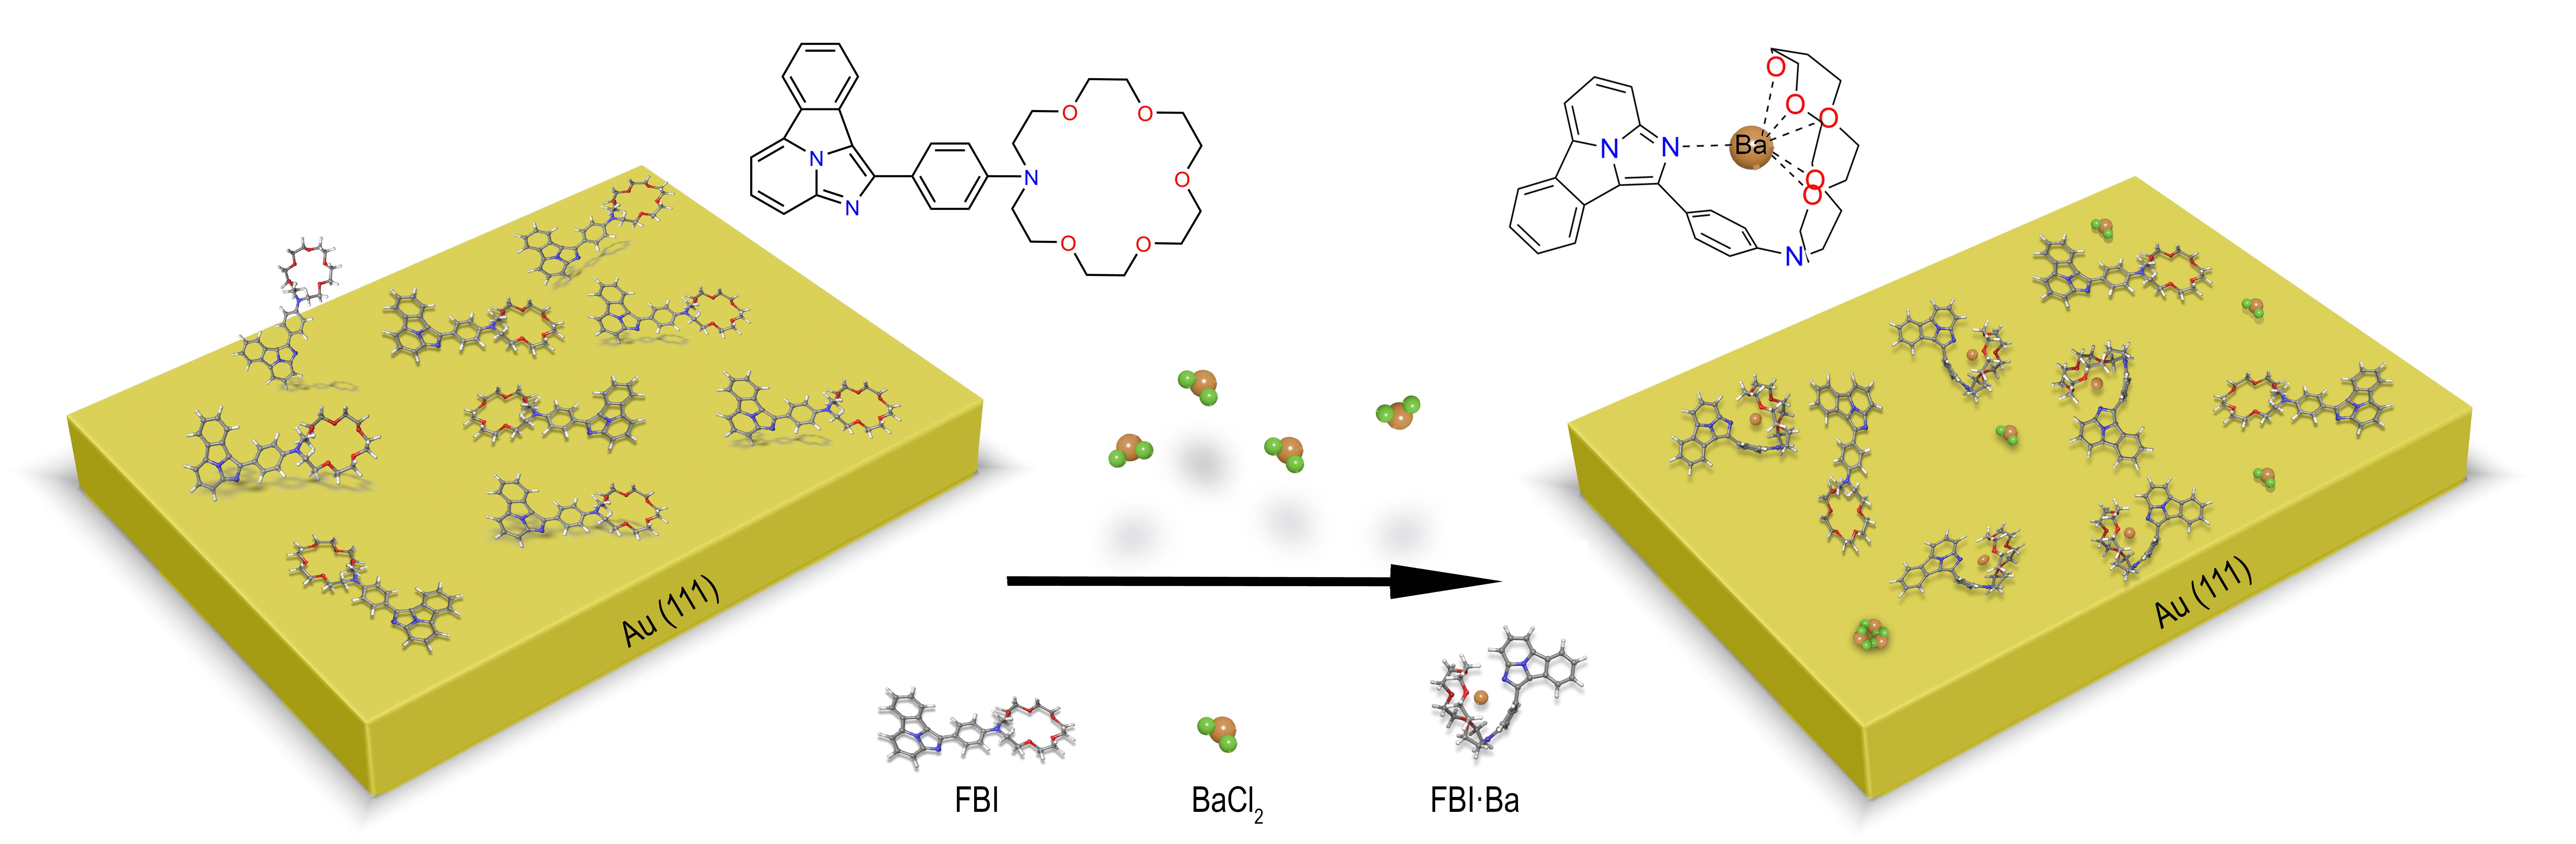
\includegraphics[width=0.9\textwidth]{figures/figura_1a.jpg}
	\caption{\label{ModeloFBI} 
    Model of the FBI molecules before and after chelation and schematic representation of the experiment we have carried out: FBI molecules were sublimated on a surface, chelated in-situ and characterized inside the UHV chamber.}
\end{figure*}  

%\section{Results and discussion}

\section{Molecular sublimation in vacuum}

In order to characterize the ion trapping capability of the FBI molecules, first it is mandatory to deposit these FBI molecules on a surface by sublimation in UHV and characterize them structural and chemically. Thus, we chose a gold substrate, the Au(111) face (single crystal cut to present (111) close-packed planes parallel to the surface), because it is a well known noble metal surface where very low substrate-molecule interaction was expected. To determine their chemical composition, we used XPS. It is worth mentioning that, since XPS sensitivity is limited to the last few nanometers, molecular coverages below 1 monolayer (ML) were always used in this study to ensure access to the substrate core levels for calibration. 

Figure {\ref{XPS_FBI_Au}}a shows the XPS spectra of the three molecular core levels of FBI, i.e. O 1s, N 1s and C 1s. The spectra were measured for 0.6 ML deposited on Au(111) at room temperature (RT). The C 1s core level can be fitted using two components, one {centered} at around 284.7 eV and a second and more intense one at 286.3 eV. The former component corresponds to C-C bonds whereas the component at higher binding energy (B.E.) includes contributions from C-O and C-N bonds, with their relative intensities in agreement with having intact molecules. In the N 1s region, around 400.4 eV, a faint peak is visible. The position of the maximum is compatible with the {enamine-imine} groups of the molecular composition. Finally, the O 1s core level presents a single component peak centered at 533.0 eV, which is compatible with previous reports on closely related crown ether groups\cite{stredansky_-surface_2019}. The ratios between the core levels, C/O = 6.2, C/N = 10.3, are in agreement with having stoichiometric molecules on the surface $ \mathrm{C_{31}N_{3}O_{5}H_{35}}$. 

In addition to the XPS analysis, we have confirmed the intact sublimation of the molecules by STM. Deposition of a submonolayer of FBI resulted mostly in disordered islands, coexisting with isolated molecules (figure {\ref{FIG_BRSTM}a}). STM images of the single molecules (inset in Figure  {\ref{FIG_BRSTM}a}) show two main triangular-like lobes. Based on the molecular structure, one of them corresponds to the fluorophore and the other to the crown-ether moieties bonded to the phenyl ring. The apparent height of both is different, with one of them appearing lower and flatter than the other. In order to correlate the apparent molecular shape and the molecular structure, bond-resolved STM images were taken. For that, the STM tip was functionalized with CO molecules operating in the repulsive tip-sample interaction regime, method extensively used in STM field for characterizing planar organic molecules \cite{gross_recent_2011,gross_atomic_2018}. Application of this measurement mode to the FBI results in the images displayed in figure \ref{FIG_BRSTM}b. On the right, the internal bonding structure of the fluorophore is approximately resolved, while the aza-crown ether regions is not well resolved. Due to its larger conformational flexibility and its non-planarity, the tip stability is not good enough and, as a consequence, the contrast observed in the aza-crown ether part is an artefact related to excessively strong interactions with the flexible CO tip-apex.\cite{moll_mechanisms_2010,hapala_mechanism_2014}. To confirm the imaging signature of the fluorophore, we also sublimated two FBI derivatives specifically synthesized without the aza-crown ether component. Figure \ref{FIG_BRSTM}c and d show the bond-resolving images of FBI derivatives sublimated on Au(111) surface: the fluorophore (figure {\ref{FIG_BRSTM}c}) and the fluorophore with the phenyl ring but without the aza-crown ether (figure {\ref{FIG_BRSTM}d}). The absence of the aza-crown ether allowed the molecules on the surface to adopt a planar, rigid conformation. This clearly improved the clarity of the images, with the carbon framework of the molecule well visualised. In turn, this supports our previous assignment of the different parts when measuring the original FBI molecules and confirms their unchanged chemical structure upon sublimation.  

\begin{figure*}[ht!]
	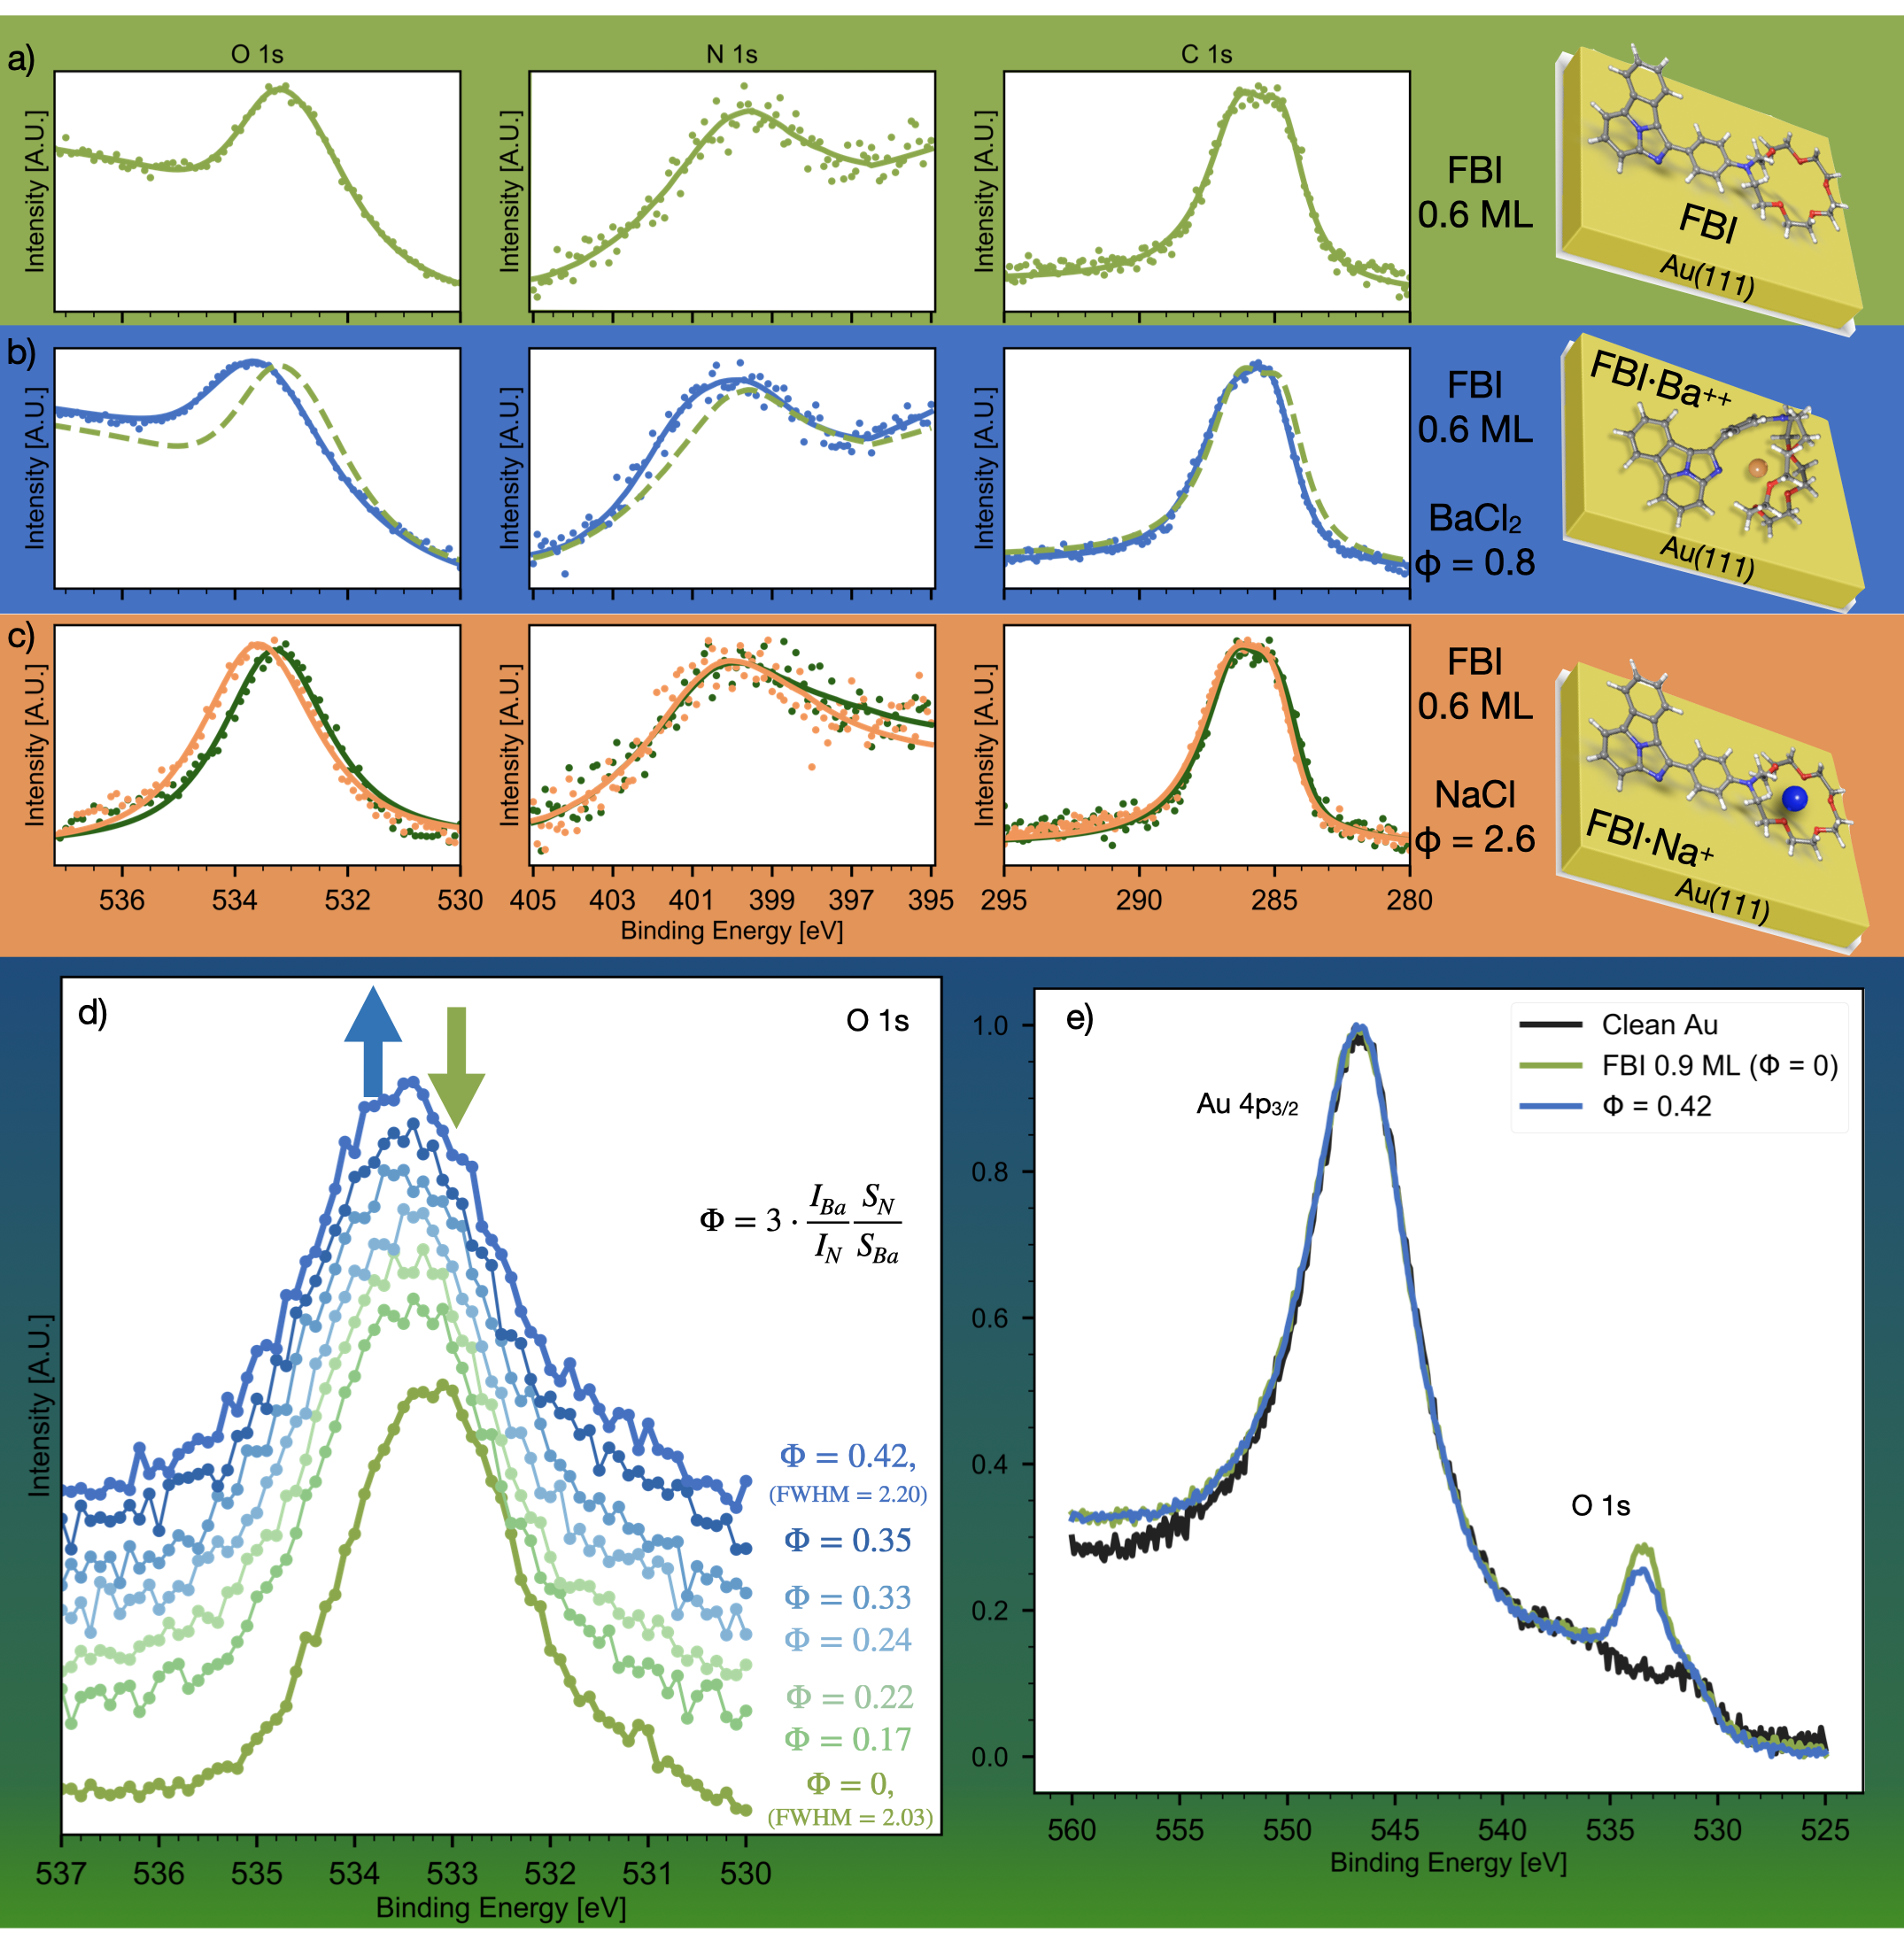
\includegraphics[width=0.99\textwidth]{figures/Figure_2.png}
	\caption{\label{XPS_FBI_Au} 
    XPS demonstration of the chemical changes induced by the molecular chelation: (a) O 1s, N 1s and C 1s core level spectra measured after sublimation of 0.6 ML of FBI deposition on Au(111); (b) O 1s, N 1s and C 1s core level spectra measured on the previous sample after chelation with 0.80 \Bapp ions per FBI molecule; (c) O 1s, N 1s and C 1s core level spectra measured after 0.6 ML of FBI deposited on Au(111) (green spectra) and after chelation \Nap\ (2.60 \Nap ions per FBI molecule) (orange line). For the three pannels dots correspond to raw values and solid lines to fitted curves (the fitting procedure is discussed in Methods section). (d) Evolution of O 1s core level as a function of the \Bapp deposition on 0.9 ML of FBI on Au(111). The spectra were manually shifted in the y-axis to better show the evolution. The O 1s core level region is displayed in d) after subtraction of the contribution from Au 4p 3/2, in order to emphasize the spectral changes in the series; (e)  Au 4p 3/2 and O 1s shown previous to any data treatment.}
\end{figure*}  

\begin{figure*}[ht!]
	\includegraphics[width=0.99\textwidth]{figures/Figure_3.png}
	\caption{\label{FIG_BRSTM} 
    (a) Large scale STM image ($50\times50$ nm$^2$) of around 0.4 ML of FBI molecules deposited on Au(111) surface and measured at 4K. Red squares show isolated molecules. Inset: constant current zoom STM image of a FBI molecule (I = 60 pA / U = 1.4 V) deposited on Au(111). (b-d) Bond-resolved STM image measured with a CO-functionalized probe (constant height, U = 5 mV) of individual FBI derivative molecules: (b) benzo[a]imidazo[5,1,2-cd]indolizine fluorophore with phenyl ring and aza-crown ether (exactly the same molecule shown in the inset in (a)); (c)  benzo[a]imidazo[5,1,2-cd]indolizine fluorophore; (d) benzo[a]imidazo[5,1,2-cd]indolizine fluorophore with phenyl ring but without the crown ether (d). For clarity a, the same image is shown twice, one with and one without the molecular model superimposed to guide the eyes.}
\end{figure*}

\section{Chemical demonstration of chelation}

Once confirmed the presence of intact FBI molecule on the surface, \BappCl\ was sublimated to test the molecular chelation. Prior to the sublimation on the FBI, \BappCl\ was sublimated on clean Au(111) surface to confirm its stoichiometry. By comparing the core level intensities of Ba 3d 5/2 and Cl 2p core levels (taking into account the corresponding sensitivity factor of each element), the ratio Ba:Cl was 1:2 as expected. Surprisingly, when \BappCl\ was deposited on FBI-functionalised Au(111), this ratio was around 1:1.5$\pm{0.2}$, meaning that some chlorine atoms desorbed when they reach the sample. From simulations \cite{rivilla_fluorescent_2020}, the chloride ions are expected to behave as passive spectators in the chelation, which is consistent with their desorption when the FBI molecule trapped the \Bapp. Because of this lack of stoichiometry, we refrain from using \Bapp\ ML to refer to the amount of sublimated molecules and, instead, we will refer the \Bapp\ ions per FBI molecule. The \Bapp\ dose was estimated using the ratio between XPS intensities of the Ba 3d 5/2 and N 1s core levels divided by the corresponding sensitivity factor, and always taking into account that there are 3 N atoms per molecule.

After sublimation of 0.80 \Bapp\ ions per FBI molecule, molecular the core levels slightly shift, which indicates changes in the chemical environment. Figure {\ref{XPS_FBI_Au}b} shows the O 1s, N 1s, and C 1s, where shifts toward higher B.E. are distinguished, mainly on O 1s and N 1s. The O 1s core level exhibits an upward chemical shift of 0.5 eV (0.4eV for N 1s). By curve fitting deconvolution (discussed in Methods section) we determine that this shift is not just a doping shift, but a real chemical change, induced by the growth of a new component. This is confirmed by the evolution of the O 1s for very low \Bapp\ doses on the surface. Figure {\ref{XPS_FBI_Au}d} shows the evolution of the O 1s for incremental amounts of \Bapp ions from 0 to almost 0.5 \Bapp\ ions per FBI molecule, i.e. up to about 2 FBI {molecules} per 1 \Bapp. Once \BappCl is added to the sample, in the O 1s core level a second component grows at higher binding energy, which induces an increase of the peak width. At the latest stage of barium addition, the FWHM increases by 9\% with respect to the initial state, which indicates that extra component appears. We deconvoluted the peaks after \Bapp\ addition using two components, one at 533.2 eV (FWHM = 2.20), corresponding to the FBI molecules and another at around 533.9 eV, consistent with the molecules undergoing a chemical change upon chelation, as previously observed for crown ether chelation with Na \cite{stredansky_-surface_2019}. It is important to mention the difficulty of quantifying correctly the variation of one component with respect to the other for O 1s. This is due to the close proximity of the Au 4p core level, Figure {\ref{XPS_FBI_Au}d}, with a contribution in the O 1s region.

To evaluate whether the nature of the ions has any influence in the oxygen core level shift for the FBI molecules, we tested the chelation with \Nap. Thus, figure {\ref{XPS_FBI_Au}c} shows the O 1s, N 1s and C 1s core levels measured on 0.6 ML of FBI on Au(111) before and after the sublimation of 2.60 \Nap per FBI. The maximum of the O 1s core level shifts again for \Nap-chelated FBI molecules 0.5 eV toward higher B.E., confirming that O 1s shift can be consider a fingerprint of the chelation. Moreover, there is no apparent shift on the N 1s (nor C 1s) core level, which reveals that N 1s is not playing any role in the chelation process. According to theoretical calculations, upon chelation with \Bapp, FBI undergoes a structural torsion generated by the interaction between the ion, the iminic N atom of the benzo[\textit{a}]imidazo[5,1,2-\textit{cd}]indolizine moiety and the phenyl group of the unbound fluorophore \cite{rivilla_fluorescent_2020}. On the contrary, in the case of \Nap\ calculations do not show such an important molecular distortion because of the smaller size of the ion. Thus, this difference between \Bapp\- and \Nap-chelation can be interpreted as a first proof that the molecular conformation of FBI and the cation-phenyl interaction varies depending on the nature of the trapped ions. 

\section{Molecular structural rearrangement induced by chelation}

\begin{figure*}[ht!]
	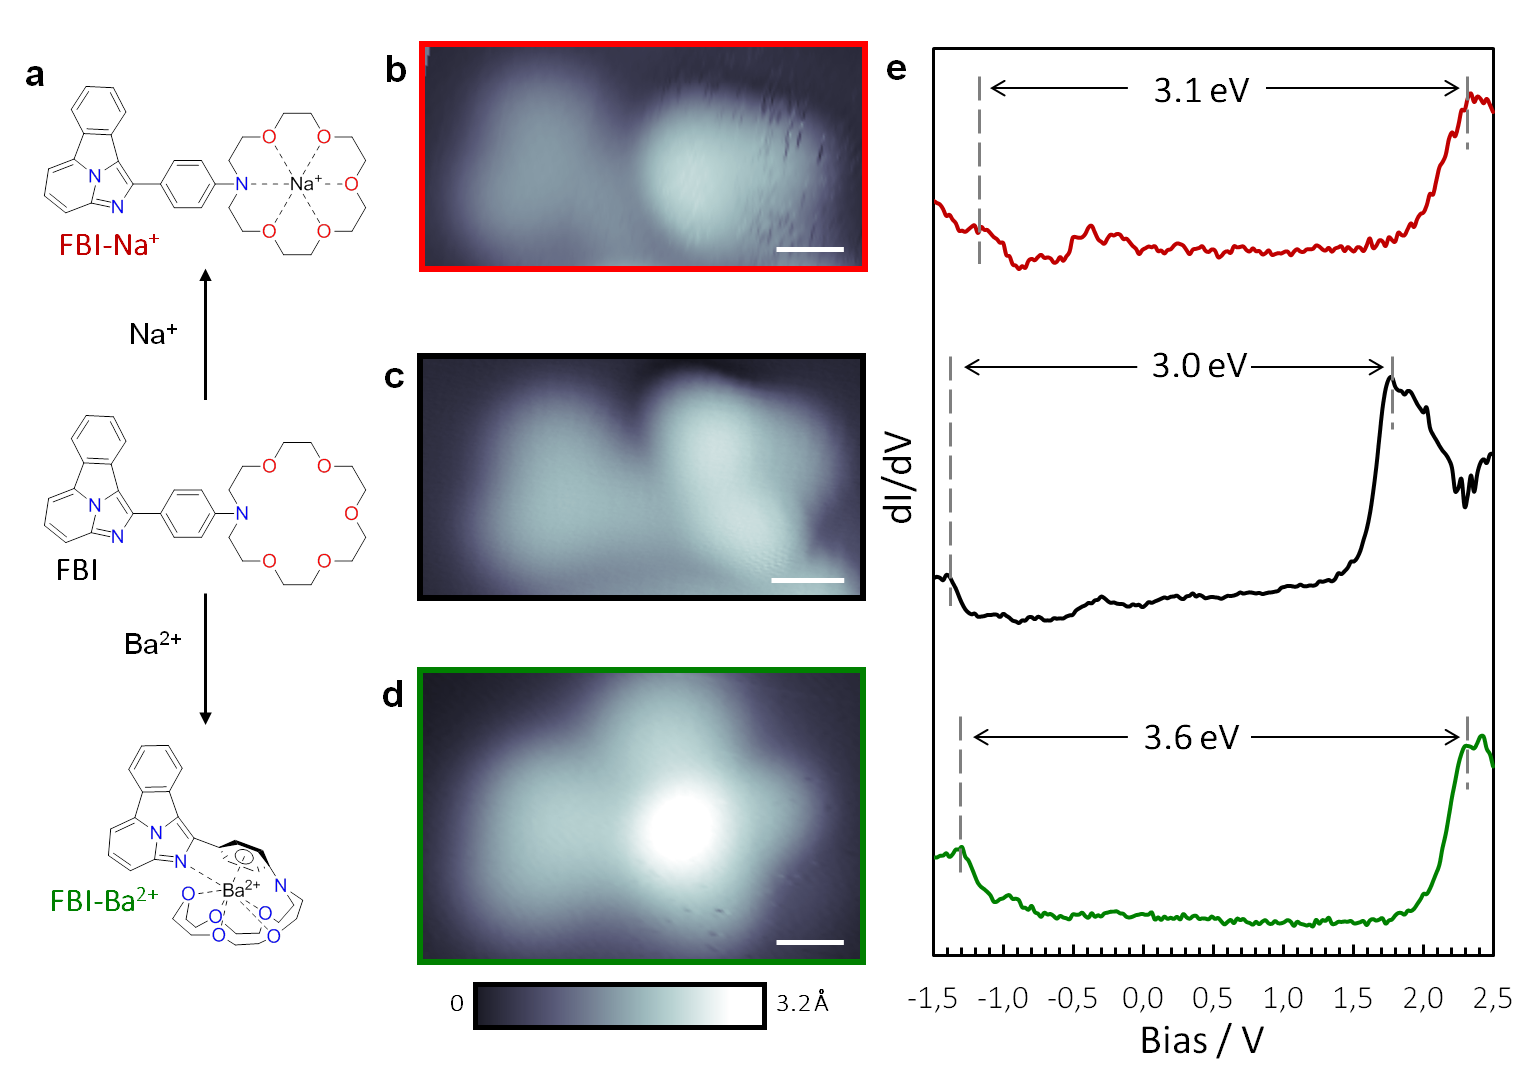
\includegraphics[width=0.9\textwidth]{figures/Fig_STS.png}
	\caption{\label{Fig_STS} 
    (a) Schematic diagram of metal intercalation. (b-d) STM images of (b) \Nap-complexed (U = 0.9 V, I = 60 pA), (c) native (U = 1.4 V, I = 60 pA), and (d) \Bapp-complexed (U = -1.8 V, I = 20 pA) FBI. (Scale bars = 0.5 nm) (e) STS spectra of native (dark), \Nap-complexed (red), and \Bapp-complexed (green) FBI.}
\end{figure*}

In order to visualize the aforementioned structural changes undergone by the FBI molecules upon chelation, 
 STM experiments were, again, carried out. Figure \ref{Fig_STS}a shows the schematic representation of the FBI molecules before and after chelation with \Nap and \Bapp, and Fig. \ref{Fig_STS}b-d displays representative STM images next to each of the cases. In all of them, the fluorophore and the aza-crown ether region are distinguished. The \Nap chelated FBI image remains almost unchanged compared to the non-chelated FBI, while the FBI chelated with \Bapp\ has a more complex shape. Although the interpretation of constant current mode STM images is always difficult because the contrast is determined by a convolution of topographical and electronic contributions, here we can directly relate the images differences with the expected conformational changes because the images were measured at bias voltages well inside the molecular gap, i.e., with no variation in the electronic structure. Taking into account that the three STM images are plotted with a common color code, it can be directly observed that the apparent heights of the crown ether follow the expected trend. Indeed, the apparent height for each of the molecules, as measured on the highest point of the crown, is 2.5$\pm$ 0.1 \AA, 2.1$\pm$ 0.1 \AA, and 2.9$\pm$ 0.1 \AA, for the pristine FBI and the \Nap and \Bapp chelated molecules, respectively. Thus, complexation of crown ethers with alkali metals like \Nap\ causes the oxygen atoms to point to the center, forcing the ring to adopt a flatter conformation relative to the native molecule. Instead, FBI molecule adopts a more three-dimensional conformation upon chelation with \Bapp.  
 
\begin{table}[]
    \centering
    \begin{tabular}{|c|c|c|c|c|}
        \hline
        Species &  Band gap / eV (nm) & $\lambda_{max}^{abs}$ / \text{nm} & $\lambda_{max}^{emi}$/\text{nm} \\ \hline
        FBI & 3.0 (413.3) & 432.5 & 489 \\
        FBI-\Nap & 3.1 (400.0) & 430 & 489 \\
        FBI-\Bapp & 3.6 (344.4) & 420.5 & 428 \\ \hline
    \end{tabular}
    \caption{Band gap values measured by STS on Au(111) vs absorption ($\lambda_{max}^{abs}$) and fluorescence emission ($\lambda_{max}^{emi}$) spectral peaks measured in solution.}
    \label{tab:bandgaps}
\end{table}

More importantly, this molecular distortion upon metal coordination has an important impact in the fluorescense response. According to calculations \cite{rivilla_fluorescent_2020}, the lowest fluorescence state of the unbound FBI molecule can be mainly characterized as the electronic transition between the Highest Occupied Molecular Orbita (HOMO) and the Lowest Unoccupied Molecular Orbital (LUMO) while the torsion of the phenyl group decreases the effective conjugation, increasing the symmetry allowed $\pi \rightarrow \pi^*$ gap, thus resulting in the blue shift of the fluorescent emission. In order to confirm this, complementary, scanning tunneling spectroscopy (STS) measurements were done. STS allows to scan the local density of states of the system. Figure {\ref{Fig_STS}e} shows the associated STS spectroscopy measured for the three molecules. The FBI molecule deposited on Au(111) has an HOMO-LUMO gap of 3.0 eV, complexation with \Nap\ did not considerably change this band gap, while complexation with \Bapp increased it to 3.6 eV. A simple complexation between the crown ether and \Nap\ therefore does not change the molecular gap substantially. This is in line with other dyes containing the same crown ether whose emission profiles do not change upon \Nap\ complexation\cite{ast_high_2011}. Meanwhile, the conformational change upon complexation with \Bapp causes a decrease in the extent of $\pi$-conjugation, which no longer extends into the phenyl ring linking the fluorophore and the crown, consequently increasing the bandgap.  Although, emission experiments can not be done for this samples because our substrate is a conductor and thus, the fluorophores are strongly quenched because the excitation energy is dumped to the metal without further emission, the measured HOMO-LUMO gap values are in line with the observed changes in absorption and emission spectra measured in solution, as summarized the Table \ref{tab:bandgaps}.


\section{Chelation independent of the surface support}


\begin{figure*}[ht!]
	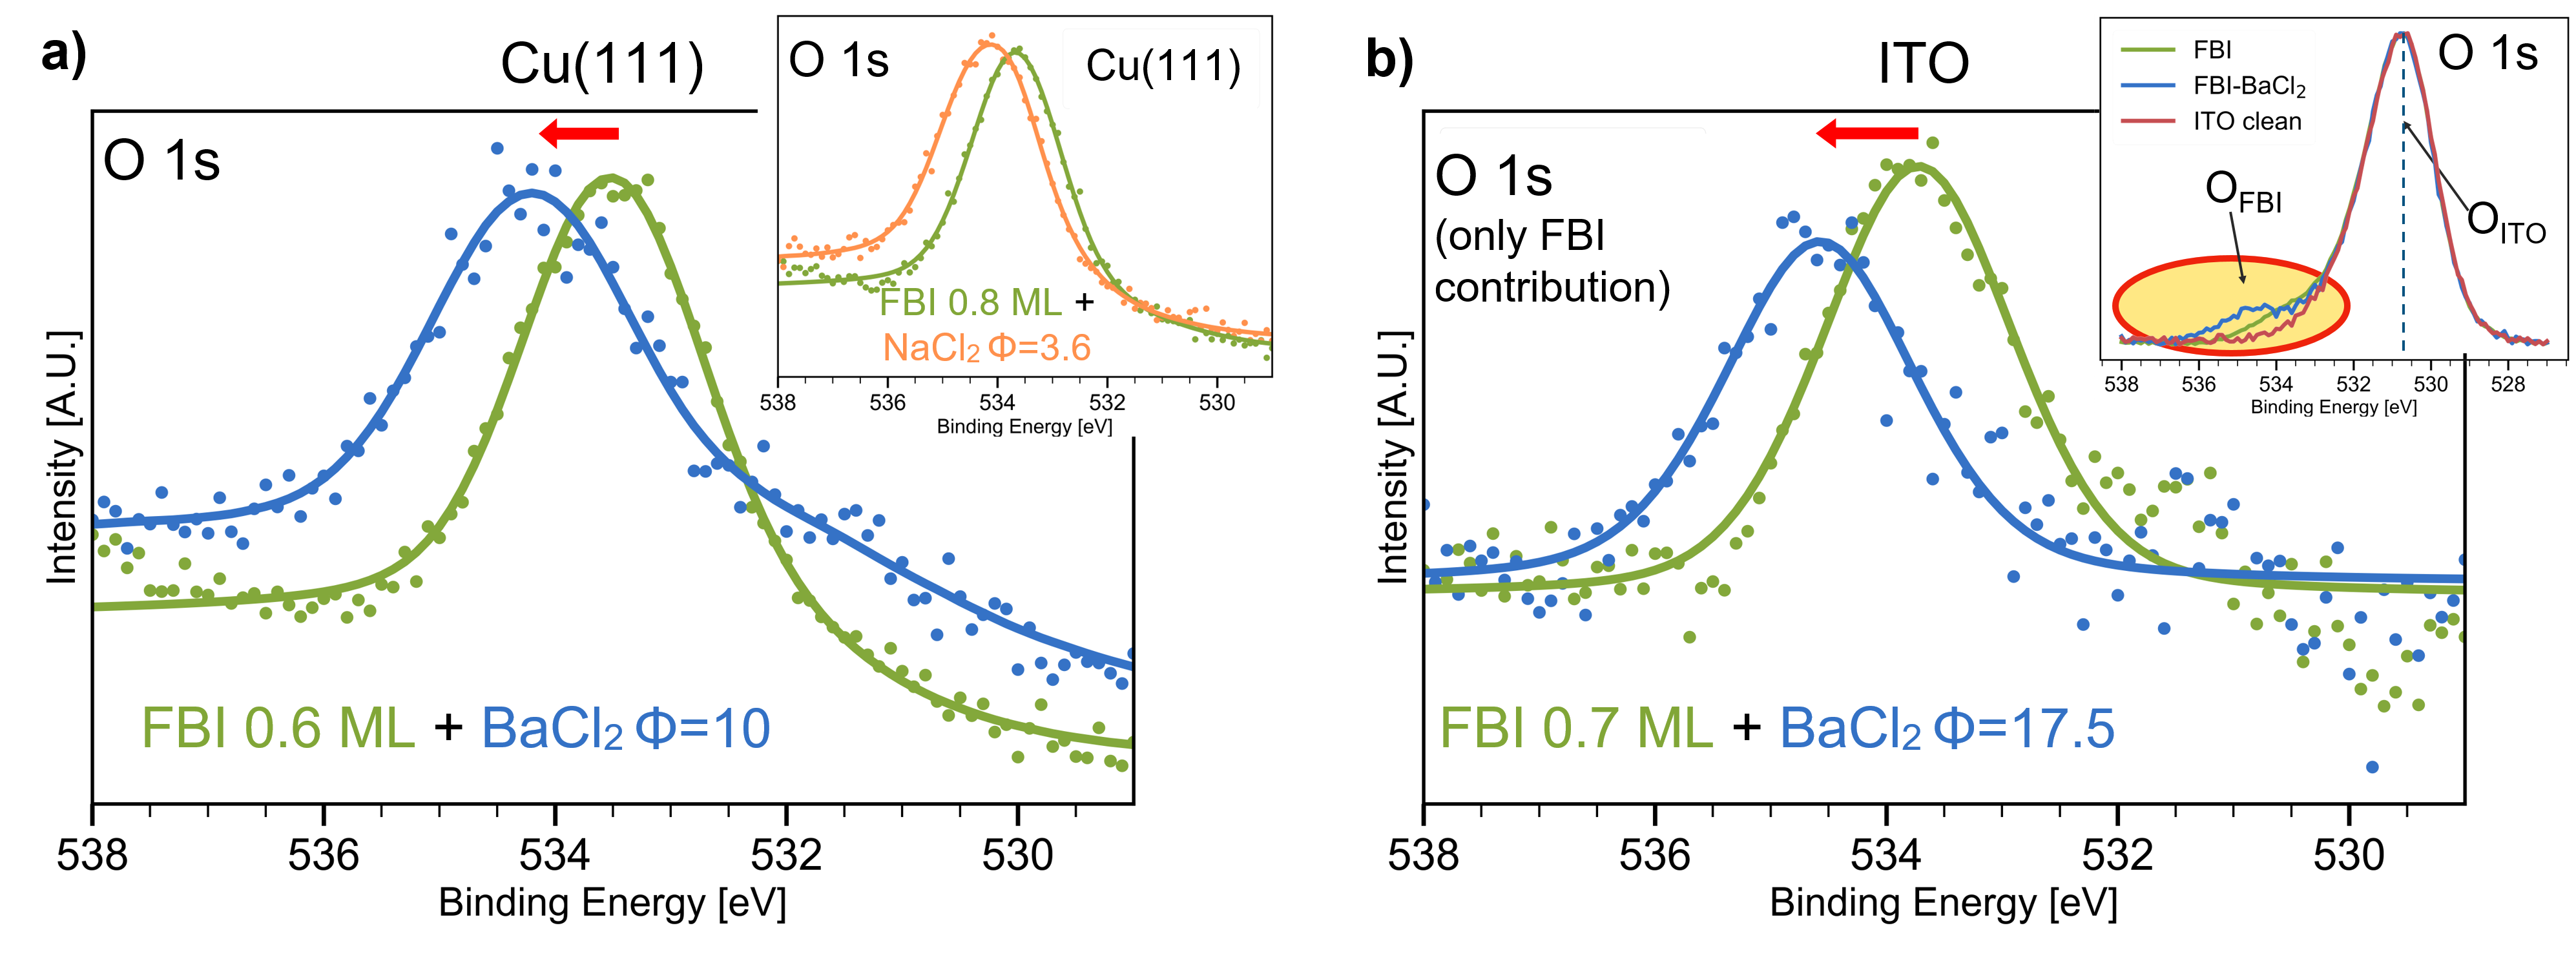
\includegraphics[width=0.95\textwidth]{figures/Figure_5.png}
	\caption{\label{XPS_FBI_Cu_ITO} 
    O 1s core level evolution upon chelation measured on two submonolayer FBI-functionalized surfaces: (a) chelation on Cu(111) sublimating \BappCl and NaCl (inset); (b) chelation on ITO. For this substrate, the substrate component (${O_{ITO}}$) was substrates to emphasize the O 1s contribution coming from FBI (${O_{FBI}}$). The entire spectra are shown inserted in (b). Dot spectra correspond to raw values and solid lines to fitted curves.}
\end{figure*} 

Finally we have also tested that chelation takes place also at other surfaces, in particular Cu(111) and ITO. We chose Cu(111) because it is a more reactive substrate. This enabled us to study whether the molecule-substrate interaction could alter the chelation response. On the other hand, ITO was selected as a promising candidate for the potential implementation of a barium tagging detector on a xenon-based TPC \cite{rivilla_fluorescent_2020}. ITO is transparent, which would allow the direct detection of fluorescence in transmission. Furthermore, its conductivity is high enough to guide the \Bapp\ ions towards the sensor surface facilitating their capture by the FBI. 

As previously discussed, the O 1s shift is a fingerprint of chelation. Figure \ref{XPS_FBI_Cu_ITO} shows the O 1s core level of FBI on Cu(111) and ITO. In both cases, upon chelation with \Bapp\ ($\phi = 10$ for 0.6 ML of FBI on Cu(111) and $\phi = 17.5$ for 0.7 ML of FBI on ITO) we observed the chemical shift on the O 1s towards higher B.E., indicating that chelation is happening. In the case of Cu(111) the shift is of about 0.7 eV while for ITO is around 0.9 eV. In the case of Cu(111) chelation was \Nap\ was also tested and, again, O 1s shows the expected upward shift associated to chelation (inset in Figure \ref{XPS_FBI_Cu_ITO}). These results ensure that chelation is independent from the choice of substrate.

The exact values of the O 1s core level shift are different for the three samples. In photoemission, the absolute core level shift values depends on many factors such as the substrate, the molecular coverage, the presence of defects or other molecules... Therefore, what is important here is that the direction of the shifts is the same in the three cases, and magnitude of the shift is similar. 

Notice that in the case of Cu(111), when FBI-functionalized surface is exposed to \BappCl, the residual contamination partially oxidized the surface. For this reason, the core level has a smaller component at lower B.E., around 531 eV, associated to  Cu$_2$O \cite{zhu_surface_2013}. Moreover, because of the presence of oxygen in the ITO structure, the analysis of the O 1s core level shifts required a subtraction of the core level measured on the bare ITO to enhance the FBI and \Bapp\ chelated FBI contributions. The result of the subtraction is shown in figure \ref{XPS_FBI_Cu_ITO} b), and the inset gathers the original normalized spectra, including the contribution to the  O 1s coming from the ITO.  



\section{Conclusions}
The demonstration of chelation in vacuum of FBI indicator by \Bapp\ ions once the molecules are deposited on suitable surfaces supports the barium tagging concept to achieve extremely low background xenon-based \bbonu\ detection experiments. Chemical and conformational changes occur upon chelation, independently of the substrate where molecules were deposited. These changes are furthermore in agreement with the calculations for the behaviour of free standing molecules, thus providing considerable freedom to choose the substrate. Moreover, the measured variation in the molecular HOMO-LUMO gap are perfectly consistent with the observed bicolour property of the sensor for \Bapp\ ions compared to the absence of shift observed and predicted for other ions, such as \Nap.  

Furthermore, this study has also important implications beyond neutrino particle physics field. The capability of {aza-crown ethers} to interact with many different ions is very important in applications such as drug carriers \cite{uchegbu_non-ionic_1998} or photo-switching devices \cite{malval_photoswitching_2002,uda_membrane_2005}. 


\section{Methods}
The experiments were performed in two different UHV chambers, one for XPS experiments and the other for STM experiments. In both cases chambers has a base pressure of $1\times10^{-10}$ mbar. Prior to deposition, the Au(111) and Cu(111) and Indium Tin Oxide (ITO) surfaces were cleanned via cycles of Ar sputtering and annealing to 500°C and their cleanness was checked by XPS prior to molecular deposition. 

\textbf{Molecular evaporation}
Pure FBI, \BappCl and NaCl powders were evaporated from homemade Knudsen cell evaporators. To avoid cross-talking between FBI and the salts molecules and to exclude any possibility of chelation of the molecule inside the cell, the FBI and \BappCl (NaCl) evaporators were located in two separated parts of the UHV chambers. To ensure the reproducibility of sublimation, molecular evaporators containing the FBI, \BappCl and NaCl were removed from one chamber and inserted in the other.  

FBI molecules were synthesized using the procedure described in \cite{rivilla_fluorescent_2020}, while \BappCl and NaCl were commercially (Sigma-Aldrich) available. The molecules were used after degassing in UHV.
The molecular evaporation rate was monitorized using a quartz microbalance and, the amount of molecules on the surfaces was afterwards quantified by analyzing the relative intensity of the core level peaks for the experiments done in XPS as well as with the percenteage of covered surface in STM. 

\textbf{Adsoption and emission spectra}
 Uv-vis spectra were acquired on a Shimatzu UV-2600 Spectrophotometer. Emission spectra were acquired on an Agilent Cary Eclipse Fluorescence Spectrophotometer. Excitation and emission monochromator bandwidth was fixed at 5 nm. Spectra were recorded at $5\times10^{-5}$ M solutions of FBI and equimolecular quantities of the corresponing perchlorate cation salt for the chelated species. Emission spectra were acquired using 250 nm light.

\textbf{STM experiments}
STM experiments were performed with a commercial Scienta-Omicron ultra-high vacuum LT-STM at 4.3 K. W tip  was used. For topography images measured were done using constant current mode, while for bond resolution images constant height mode was used, Figure \ref{FIG_BRSTM} b-d. During the STM experiments, the tip was functionalized with CO for bond resolution STM by exposing the sample to low pressure (approximately $1 \times 10^{-8}$ mbar) of CO whilst the sample was held below 7 K. CO molecules were trapped by the tip from their adsorption sites via scanning over them or by applying $\sim$ 2 V bias voltage pulses. 

\textbf{XPS experiments}
The XPS measurements were carried out using a Phoibos-100 electron analyzer (SPECS GmbH), using a non monochromatic Al K$\alpha$ photon source, 1486.6 eV. The spectra were calibrated to the substrates main core level (Au 4f, Cu 2p, and In 3d, respectively). 

The evaporation thicknesses were estimated using the attenuation of the most intense substrate core levels, i.e. Au 4f, Cu 2p and In 3d for Au(111), Cu(111) and ITO, respectively. The calculations followed the guidelines provided in ref. \cite{powell_practical_2020}. For this purpose, we estimated the electron Effective Attenuation Length (EAL) of electrons through the FBI layers for electrons with kinetic energies of 1402.6, 1041.6 and 554.61 eV (Au 4f 5/2, In 3d 5/2 and Cu 2p 3/2). The resulting EALs are 3.87, 3.05 and 1.85 nm, respectively. The thickness of the FBI samples was then estimated using the intensity of clean substrate core level as reference and the attenuated intensity after the evaporation. 

The stoichiometry of the FBI (\BappCl) was calculating following the expression $ R(A/B)=(I_{A}/I_{B} \cdot S_B/S_{A})$ where A and B are the different molecular elements, $I_{X}$ is the integrated area under the main core level and $S_{X}$ is the corresponding sensitivity factor of this core level.

The amount of \Bapp (\Nap) per FBI molecule were estimated by computing  the ratio $\phi=I_{Ba}/(I_N/3) \cdot S_N/S_{Ba} $, where $I_{Ba}$, $I_N$ are total areas  of Ba 3d 5/2 and  N 1s core  levels, respectively, and $S_{Ba} = 25.84$, $S_N = 1.80$ are the corresponding atomic sensitivity factors \cite{scofield_hartree-slater_1976}. The factor 3 responds to stoichiometric reasons, considering 3 N atoms per molecule.

\textbf{XPS fitting}
The spectra fitting was performed using custom-made software written in Python, using the lmfit library \footnote{https://lmfit.github.io/lmfit-py/}. An example of fit can be seen in figure \ref{XPS_fits}. The CL were modeled as a pseudo-Voigt function (Lorentzian to Gaussian ratio of 0.6) convoluted with a Shirley type background. The error in the estimation of the position of the maxima associated to the fitting is 50 meV. When estimating stoichiometry, to correct for systematic uncertainties affecting different sets of data, the intensities of all spectra were rescaled to the main substrate core levels (Au 4f, Cu 2p and In 3d, respectively). The CL peak area were numerically integrated between fixed local minima. This yields an error in the stoichiometry ratios of 7\%. 


\begin{figure*}[ht!]
	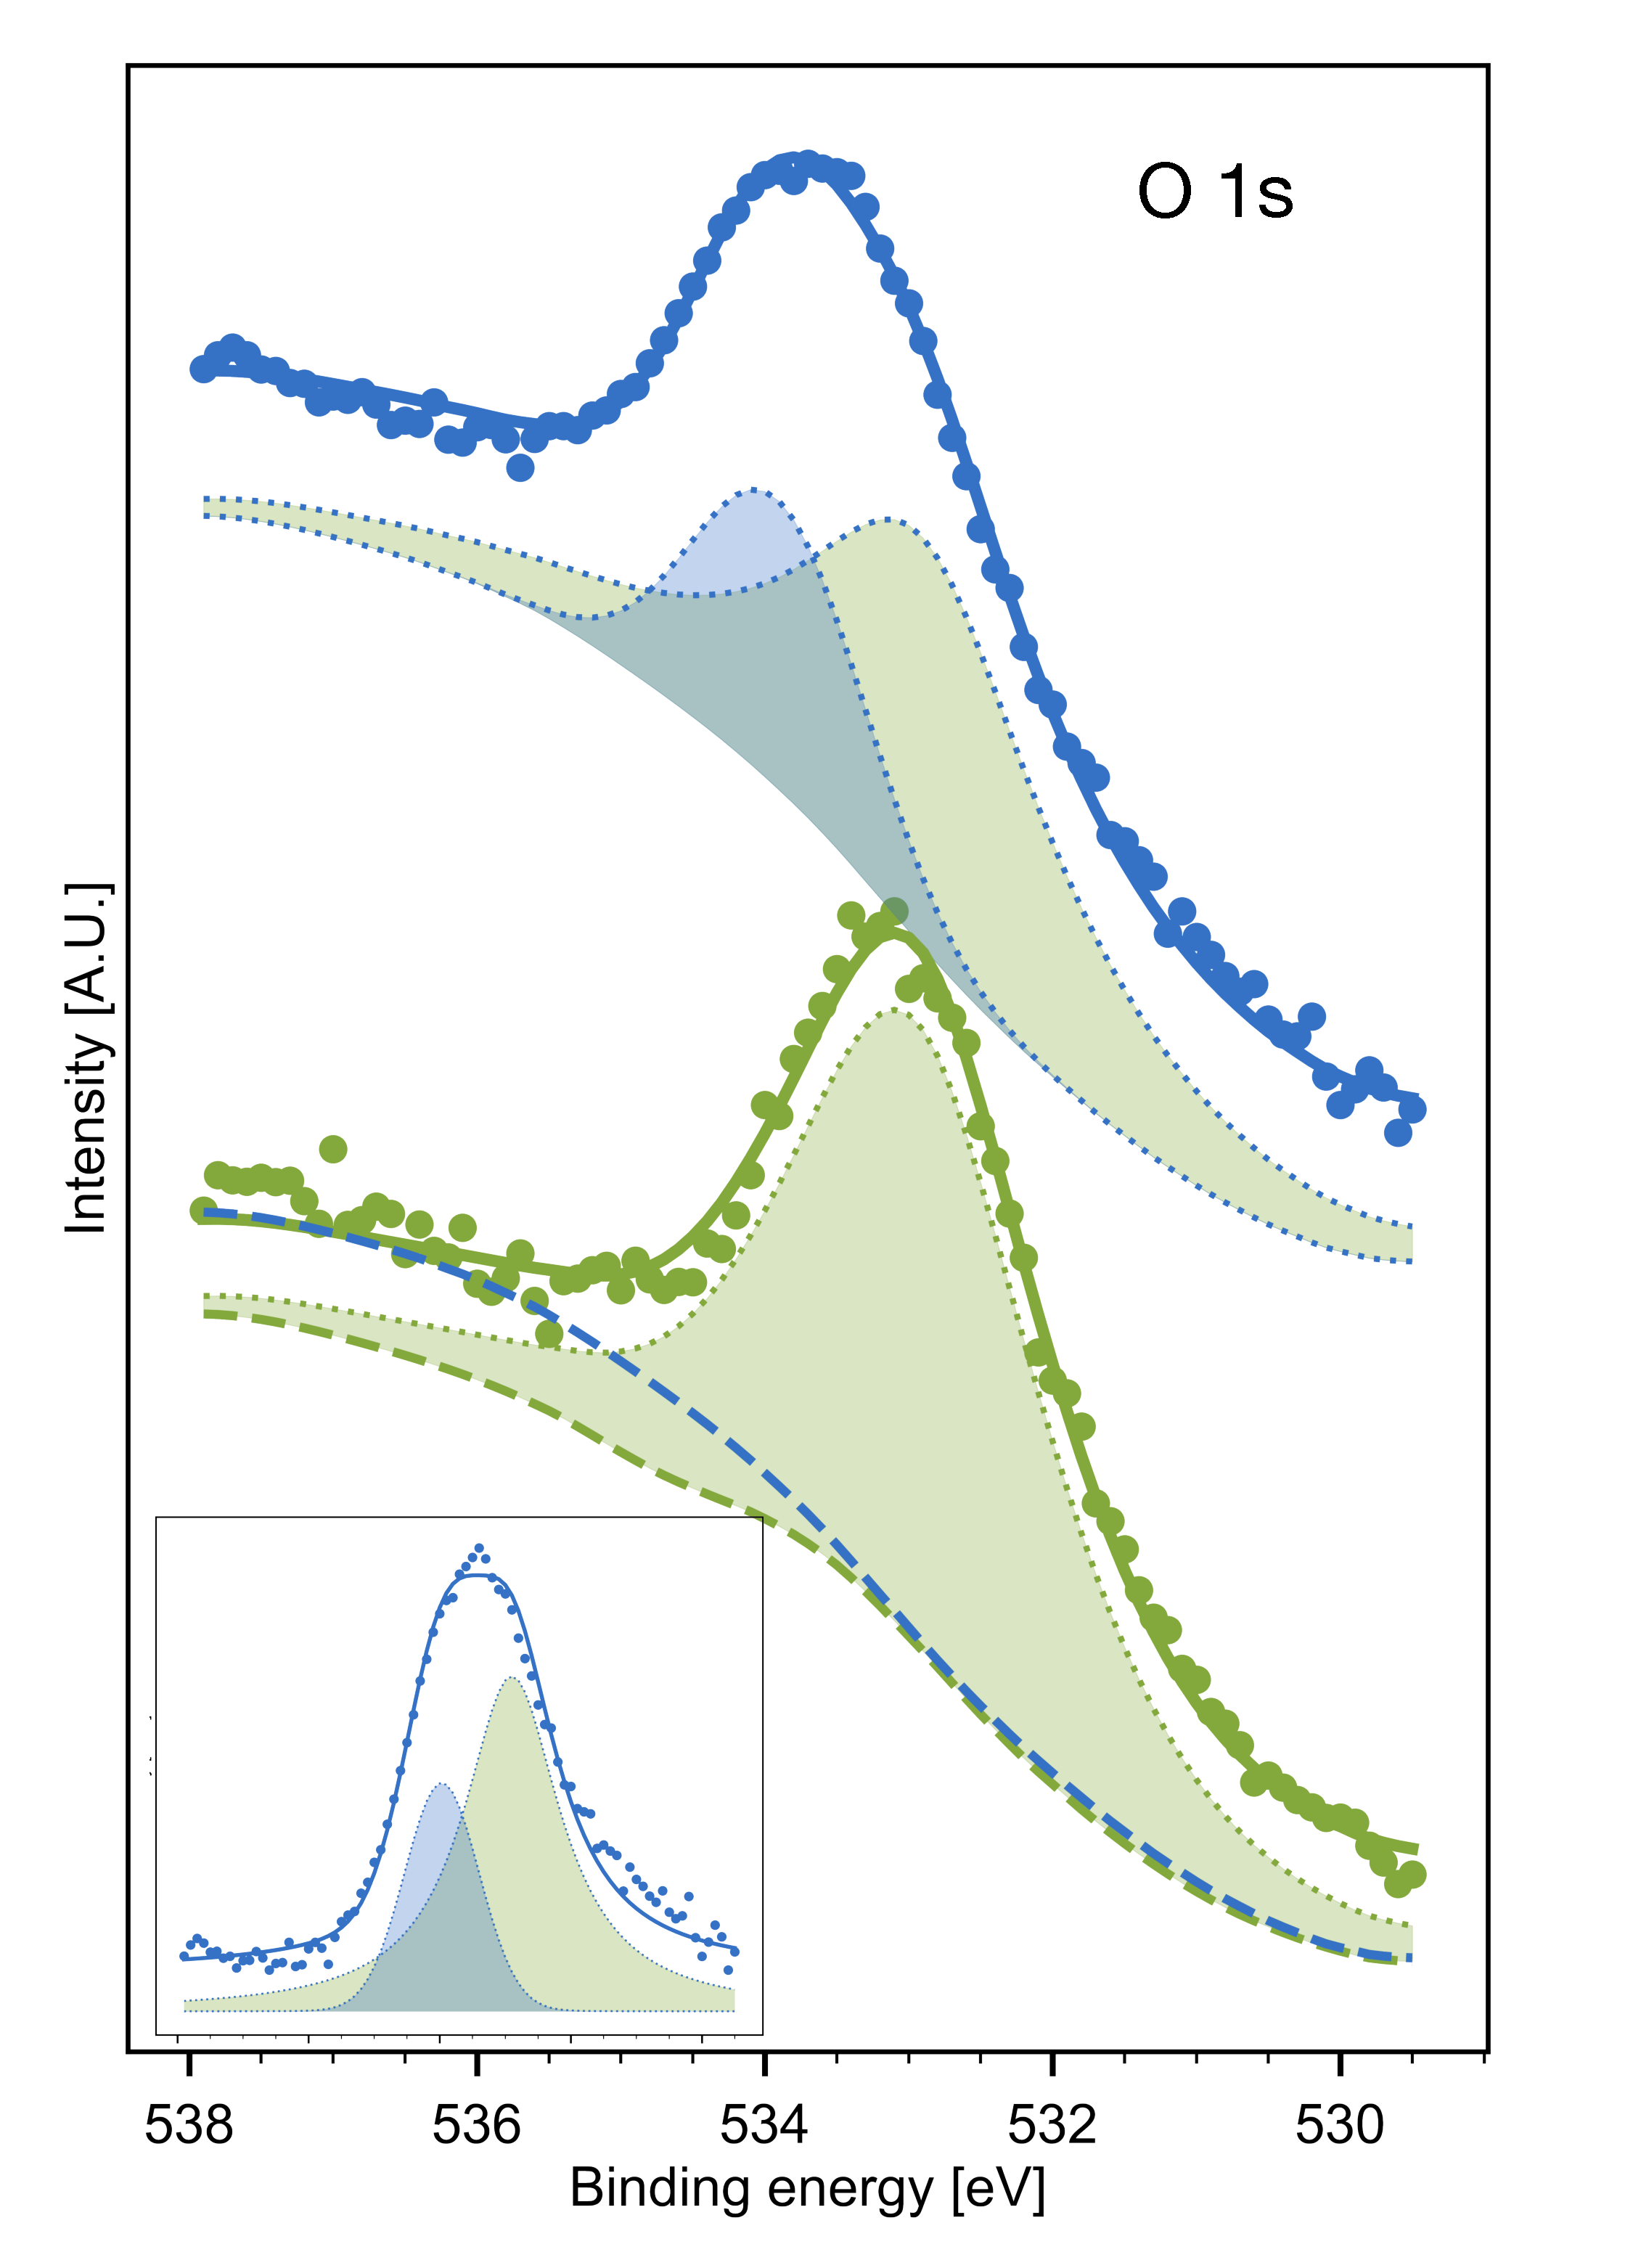
\includegraphics[width=0.45\textwidth]{figures/fig6_fit.pdf}
	\caption{\label{XPS_fits} Same as O 1s from fig. \ref{XPS_FBI_Au} a) and b) with detailed fitting components (dotted lines). Green circles and solid line: 0.6 ML FBI raw data and best fit, respectively. Blue circles and solid line: 0.6 ML FBI + BaCl$_2$, $\phi$ = 0.8,  raw data and best fit, respectively. The green component was fitted to the unchelated FBI data (green circles) at 532.95 $\pm$ 0.05 eV, with width 2.16 $\pm$ 0.04 eV at FWHM. This component was then fixed in position and width for the chelated FBI data (blue dots). An additional component was fitted to the chelated FBI CL, shown as blue filled area, at 533.91 $\pm$ 0.05 eV,  with 1.41 $\pm$ 0.05. The background of each curve is shown as dashed lines in green and blue, respectively. Inset: same blue curve and components with its background subtracted.}
\end{figure*}  

\bibliographystyle{apsrev4-1} 
\bibliography{literature_FBI}

\section{Acknowledgment}
We acknowledge support from the following agencies and institutions: European Research Council (ERC) under ERC-2020-SyG 951281; the Ministry of Science and Innovation of Spain and under grants PID2020-114252GB-I00, PID2019-107338RB-C63,  FIS2014-53371-C04, the Severo Ochoa Program
grant CEX2018-000867-S; the Basque Government (GV/EJ) under grants IT-1346-19 and IT-1180-19. 
\section{Author contributions}
J.J.G.-C., F.P.C. and C.R. conceived the project. C.R. designed and coordinated the experiments and data analysis. P.H.G. and M.I. performed and analysed the XPS experiments. J.P.C., A.B.L., T.W., D.G.O. and M.C. performed the STM experiments. R.G.M. I.R., B.A., A.A. and Z.F. carried out the chemical synthesis, and characterisation in solution of fluorescence studies. C.R., P.H.G., J.J.G.-C., F.P.C. and J.P.C. wrote the manuscript. The NEXT collaboration assisted with edition and revision of the manuscript. 

\end{document}
